\chapter{Grundlagen der EU-Erweiterung }
Ob und in welchem Umfang die EU erweitert werden soll, ist eine politische Entscheidung. Auch die zeitlichen Abläufe für den Beitritt von Staaten zur EU werden durch politische Entscheidungen dominiert, wenngleich für diesen Aspekt binnenorganisatorische Abläufe informell ebenfalls von Bedeutung sein könnten. Die Gestaltung eines Beitrittsprozesses wirft viele Fragen auf, die teils fallspezifisch, teils allgemeiner Art sind. In Betracht kommen politische, ökonomische, soziale und administrative Probleme des gewünschten oder notwendigen Wandels. \par
Prozesse des Wandels sind sowohl Gegenstand verschiedener theoretischer Überlegungen als auch eine Gelegenheit, entsprechende Praxiserfahrungen zu sammeln. Da die EU seit ihrer Gründung bereits mehrfach erweitert wurde, liegt schon ein umfangreiches Praxiswissen zu Beitrittsprozessen zur EU vor; von diesem ist allerdings nicht genau bekannt, in welchem Umfang es fallspezifisch oder wieweit es übertragbar ist.
\section{Die Erweiterung der EU in der Praxis }
Die Europäische Union in den 1950er Jahren, zunächst mit der Gründung der Europäischen Gemeinschaften, umfasste sechs Staaten (Belgien, Frankreich, Deutschland, Luxemburg, Italien und die Niederlande). Ziel war es, nach dem Zweiten Weltkrieg einen wirtschaftlichen Staatenverbund zu schaffen, der die Gefahr gewaltsamer Auseinandersetzungen vermindern und durch einen gemeinsamen Markt die Wirtschaft ankurbeln sollte. Der EU, mit den Römischen Verträgen von 1957 gegründet, gehören inzwischen 27 Länder an, die in sogenannten Erweiterungsrunden aufgenommen wurden. Länder, die geografisch zu Europa gehören und demokratisch verfasst sind, können in die EU aufgenommen werden. Die umfassendste Erweiterung wurde 2004 umgesetzt mit der Aufnahme von Zypern, der Tschechischen Republik, Estland, Ungarn, Lettland, Malta, Polen, der Slowakei und Sloweniens. In derselben Erweiterungsrunde, aber mit einer Verzögerung, traten Bulgarien und Rumänien 2007 der EU bei. Die Aufnahme Kroatiens ist für 2013 vorgesehen.\par
\renewcommand{\arraystretch}{1.5}
\begin{table}[!hbt]\vspace{1ex}
\centering
\footnotesize
\caption{Geschichte der Verträge zur Europäischen Gemeinschaft}

\begin{tabular}{|Q{12mm}|Q{12mm}|Q{4cm}|Q{7cm}|}\hline
Unter\-zeichnet &In Kraft & Name&Inhalt\\\hline
1951&1952&Vertrag von Paris&Europäische Gemeinschaft für Kohle und Stahl (EGKS)\\\hline
1957&1958&Verträge von Rom&EWG-Vertrag, Europäische Wirtschaftsgemeinschaft (EWG) und der EURATOM-Vertrag\\\hline
1965&1967&Fusionsvertrag&Einsetzung eines gemeinsamen Rates und einer gemeinsamen Kommission der Europäischen Gemeinschaften\\\hline
1986&1987&Einheitliche Europäische Akte&Binnenmarkt eingeführt\\\hline
1992&1993&Vertrag von Maastricht&Europäische Union\\\hline
1997&1999&Vertrag von Amsterdam&Änderungen des Maastrichter Vertrages\\\hline
2001&2003&Vertrag von Nizza&Änderungen der Verträge von Rom und Amsterdam\\\hline
2004& &Verfassungsvertrag&Verfassung für Europa (abgelehnt)\\\hline
2007&2009&Vertrag von Lissabon&Änderungen des Vertrages über die Europäische Union (EUV) und des Vertrages über die Arbeitsweise der Europäischen Union (AEUV)\\\hline
\multicolumn{4}{c}{}
\end{tabular}\\
{\normalsize Quelle: nach \cite{moller}: 4 (eigene Ergänzung zum Vertrag von Lissabon).}
\end{table}
\renewcommand{\arraystretch}{1.2}
\subsection{Das Verfahren zur Aufnahme eines Staates }
Die Aufnahme neuer Mitglieder war von Anfang an in der Gründungsidee der EU enthalten. In Art. 6 Absatz 1 des Vertrages über die Europäische Union (EUV) ist festgelegt: „Die Union beruht auf den Grundsätzen der Freiheit, Demokratie, der Achtung der Menschenrechte und Grundfreiheiten sowie der Rechtsstaatlichkeit; diese Grundsätze sind allen Mitgliedstaaten gemeinsam“. Artikel 49 des Vertrages legt fest: „Jeder europäische Staat, der die in Art. 6 Abs. 1 genannten Grundsätze achtet, kann beantragen, Mitglied der Union zu werden“. Über diese allgemeine Verfügung hinaus muss die EU in der Lage sein, neue Mitglieder aufzunehmen, was im Einzelfall entschieden wird. Eine Aufnahme geschieht durch Konsensbeschluss der EU-Mitgliedstaaten mittels ihrer Vertreter im Ministerrat oder Europäischen Rat. Nach dem Antrag auf Aufnahme wird aufgrund einer Stellungnahme der Europäischen Kommission entschieden, ob das Land als Beitrittskandidat anerkannt wird. Innerhalb der Kommission ist die Generaldirektion Erweiterung zuständig für Koordination, regelmäßige Berichterstattung sowie enge Zusammenarbeit mit den Line DGs und den Arbeitsgruppen des Europäischen Rates (vgl. \cite{summa}: 13). Der Delegation der EU in den Kandidatenländern kommt ebenfalls eine wichtige Rolle zu in der Koordination zwischen der Europäischen Kommission in Brüssel und den Kandidatenländern.\par
Vor der Aufnahme in die EU findet ein Prozess der Verhandlungen über unterschiedliche Politikbereiche statt, um die Übernahme des vollständigen gemeinschaftlichen Besitzstandes zu gewährleisten. Dies ist eine Aufnahmebedingung. Vor einer Aufnahme muss dann der entsprechende Vertrag in den Mitgliedstaaten nach dem dafür vorgesehenen Verfahren ratifiziert werden. Schließlich muss noch das Europäische Parlament seine Zustimmung geben (vgl. \cite{euko07}: 6f).
\par
In den Kandidatenländern wird die Arbeit im Zusammenhang mit dem Beitrittsprozess meist von einem Minister in einem bestehenden Ministerium oder aus einem eigens geschaffenen Ministerium für den Erweiterungsprozess koordiniert (vgl. \cite{summa}: 14).\par
Die Stadien im Erweiterungsprozess sind im folgenden Schema überblicksartig dargestellt:
\begin{figure}[H]
  \centering

   \caption{Phasenmodell des EU-Beitritts }
  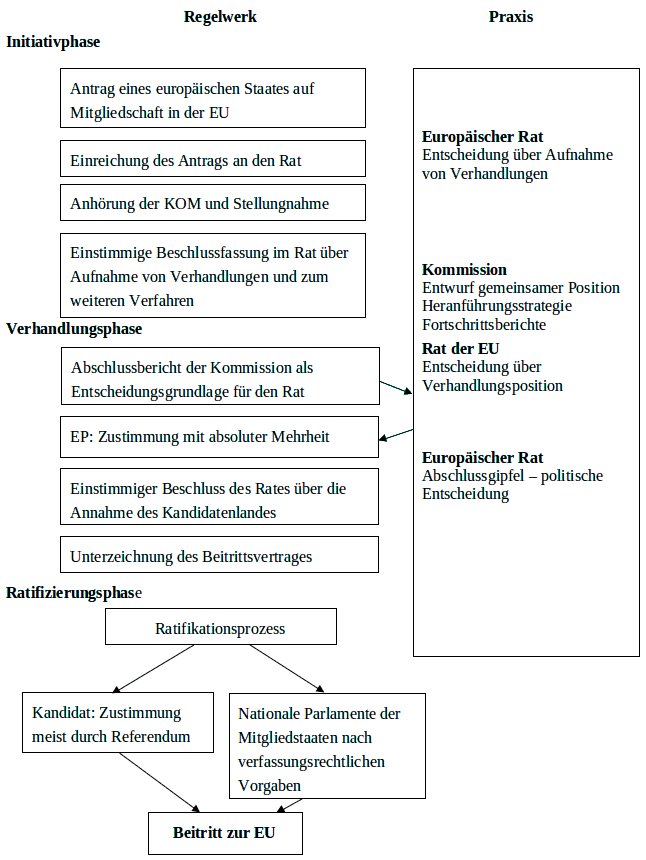
\includegraphics[width=5in]{Material/Phasenmodell_ohneRand}\\

Quelle: in Anlehnung an \cite{wessels}: 449.
\end{figure}
In der Darstellung ist der gesamte Prozess der Aufnahme in den einzelnen erforderlichen Schritten schematisch dargestellt. Dabei werden drei Hauptphasen unterschieden: Die Initiativ-, die Verhandlungs- und die Ratifizierungsphase. Der angestrebte EU-Beitritt der drei Untersuchungsländer dieser Arbeit ist aktuell geprägt von der Umsetzung und Abarbeitung der Heranführungsstrategie und der jährlichen Berichterstattung (im Schema Fortschrittsberichte genannt).\par

Nachdem ein Land offiziell den Aufnahmeantrag gestellt hat, bekommt es von der EU-Kommission einen Fragebogen zu allen Bereichen des Acquis communautaire geschickt. Diese Fragebögen zu den bestehenden Institutionen, policies und der Infrastruktur müssen von dem Antragsteller ausgefüllt und der EU-Kommission übersandt werden. Auf der Grundlage dieser Antworten erarbeitet die Kommission eine vorläufige Stellungnahme zu dem Beitrittsgesuch des Landes, mit einer Empfehlung, ob und ggf. wann das Land die Beitrittsverhandlungen beginnen kann. Um offiziell Beitrittskandidat zu werden, muss der Europäische Rat/Council of Ministers formal beschließen, mit dem Land Beitrittsverhandlungen aufzunehmen. Die Kommission tritt dann in einen Prozess des “screening” ein, in dem die Gesetzgebung und policies des Landes mit der EU verglichen werden, “in order to make longterm plans to bring applicant countries up to EU standards“ (\cite{grab10}: 3).
Die praktische Durchführung der Erweiterung ist ein komplexer Prozess, der sich evolutionär entwickelt hat. Keine Erweiterungsrunde war bisher mit der vorherigen identisch und in jedem Fall wurden neue Erweiterungsinstrumente eingeführt oder bestehende weiterentwickelt (vgl. \cite{kochenov}: 16). Die bisherigen Aufnahmen mit den Schritten vom Beitrittsantrag bis zum Beitritt sind im folgenden Schema mit der in der Literatur vorherrschenden Bezeichnung der jeweiligen Erweiterung dargestellt.\\
\begin{table}[H]\vspace{1ex}\centering
\caption{Bisherige EU-Erweiterungen}
\footnotesize
\begin{tabular}{|p{2cm}|p{2cm}|p{2cm}|p{2cm}|p{2cm}|p{2cm}|}\hline
&Beitritts\-antrag&Stellung\-nahme Kommis\-sion&Beginn Beitritts\-verhand\-lungen&Unter\-zeichnung Beitritts\-vertrag&Beitritts\-datum\\\hline
\multicolumn{6}{|p{12cm}|}{1. Norderweiterung} \\\hline 
Vereinigtes Königreich&
10.05.1967 (09.08.61)*&
19.09.1967&
30.06.1970&
22.01.1972&
01.01.1973\\\hline
Dänemark&
11.05.1967 (10.08.61)*&
19.09.1967&
30.06.1970&
22.01.1972&
01.01.1973\\\hline
Irland&
11.05.1967 (10.08.61)*&
19.09.1967&
30.06.1970&
22.01.1972&
01.01.1973\\\hline
\multicolumn{6}{|p{12cm}|}{2. Süderweiterung}\\\hline
Griechenland &
12.06.1975&
29.01.1976&
27.07.1976&
28.05.1979&
01.01.1981\\\hline
Portugal&
28.03.1977&
19.05.1978&
17.10.1978&
12.06.1985&
01.01.1986\\\hline
Spanien&
28.07.1977&
29.11.1978&
05.02.1979&
12.06.1985&
01.01.1986\\\hline
\multicolumn{6}{|p{12cm}|}{3. EFTA-Erweiterung}\\\hline
Österreich&
17.07.1989&
01.08.1991&
01.02.1993&
24.04.1994&
01.01.1995\\\hline
Schweden&
01.07.1991&
31.07.1992&
01.02.1993&
24.04.1994&
01.01.1995\\\hline
Finnland&
18.03.1992&
04.11.1992&
01.02.1993&
24.04.1994&
01.01.1995\\\hline
\multicolumn{6}{|p{12cm}|}{4. Erweiterung Mittel- und Osteuropa}\\\hline
Ungarn&
31.03.1994&
16.07.1997&
31.03.1998&
16.04.2003&
01.05.2004\\\hline
Polen&
05.04.1994&
16.07.1997&
31.03.1998&
16.04.2003&
01.05.2004\\\hline
Slowakei&
27.06.1995&
16.07.1997&
15.02.2000&
16.04.2003&
01.05.2004\\\hline
Lettland&
13.10.1995&
16.07.1997&
15.02.2000&
16.04.2003&
01.05.2004\\\hline
Estland&
24.11.1995&
16.07.1997&
31.03.1998&
16.04.2003&
01.05.2004\\\hline
Litauen&
08.12.1995&
16.07.1997&
15.02.2000&
16.04.2003&
01.05.2004\\\hline
Tschechien&
17.01.1996&
16.07.1997&
31.03.1998&
16.04.2003&
01.05.2004\\\hline
Slowenien&
10.06.1996&
16.07.1997&
31.03.1998&
16.04.2003&
01.05.2004\\\hline
Rumänien&
22.06.1995&
16.07.1997&
15.02.2000&
25.04.2005&
01.01.2007\\\hline
Bulgarien&
14.12.1995&
16.07.1997&
15.02.2000&
25.04.2005&
01.01.2007\\\hline
\multicolumn{6}{|p{12cm}|}{* In Klammern der Zeitpunkt des jeweils ersten Beitrittsantrages: In Folge des Scheiterns der Verhandlungen mit dem Vereinigten Königreich kam es ebenfalls zum Abbruch der Verhandlungen mit den übrigen Bewerbern.}\\\hline
\multicolumn{6}{c}{}
\end{tabular}\\
Quelle: \cite{wessels}: 451.
\end{table}
Aus dieser Darstellung wird ersichtlich, dass die bisherigen EU-Erweiterungen in Wellen stattgefunden haben, mit der Aufnahme von Ländern oft in Gruppen. Darauf sind auch die umgangssprachlichen Benennungen wie „EU-Süderweiterung“ oder „EU-Osterweiterung“ zurückzuführen. 

\subsection{EU-Erweiterungen in der Wahrnehmung der Öffentlichkeit}
Die Wahrnehmung der Öffentlichkeit in EU-Ländern hinsichtlich einer erneuten EU"=Erweiterung lässt deutliche Unterschiede erkennen. Dabei wird in den „neuen“ EU-Ländern eine erneute Erweiterung am positivsten gesehen und in den „alten“ EU-15 Ländern am negativsten. Weiterhin sinkt im Durchschnitt die Befürwortung einer Erweiterung um ca. 3 Prozentpunkte jährlich. In Polen wird die Erweiterung am positivsten bewertet, mit 74\% im Jahre 2008. Die Befürwortung einer erneuten Erweiterung lag im EU-Durchschnitt im selben Jahr nur bei 47\% (EU-27). In Ländern mit geringer Begeisterung der Bevölkerung für eine erneute Erweiterung, wie Österreich, Frankreich und Deutschland, stehen die Regierungen einer Südosterweiterung positiv gegenüber, ungeachtet der Einstellung der Mehrheit der Bevölkerung (vgl. \cite{mus}: 20).\par

In den Beitrittsländern, die Gegenstand der vorliegenden Arbeit sind, hat sich die Unterstützung der Bevölkerung für den EU-Beitritt unterschiedlich entwickelt. So ist in Montenegro die Zustimmung zur EU-Orientierung des Landes im Zeitraum 2009-2010 von 67\% auf 73\% gestiegen. In Mazedonien dagegen fiel die Zustimmung zu einem EU-Beitritt des Landes im selben Zeitraum von 62\% auf 60\%. Im gesamten Westlichen Balkan ist die EU-Orientierung der Bevölkerung in Albanien im Jahr 2010 mit 81\% am höchsten, hat aber dennoch 9 Prozentpunkte Zustimmung gegenüber dem Vorjahr verloren (vgl. \cite{gallup10}).\par
In einer repräsentativen Umfrage in den Mitgliedsländern der EU wird deutlich, dass die Bevölkerung dort im Zusammenhang mit einer erneuten Erweiterung vor allem Freiheit und demokratische Werte, noch vor ökonomischen Überlegungen, in Bezug auf Europa als Ganzes wichtig findet. In Bezug auf das eigene Land war den Befragten allerdings der ökonomische Aspekt der Erweiterung wichtiger, wie aus folgender Tabelle ersichtlich wird:
\begin{figure}[H]\centering
\setlength\belowcaptionskip{10pt}
  \caption{Umfrage zur EU-Erweiterung in den Mitgliedstaaten der EU }
  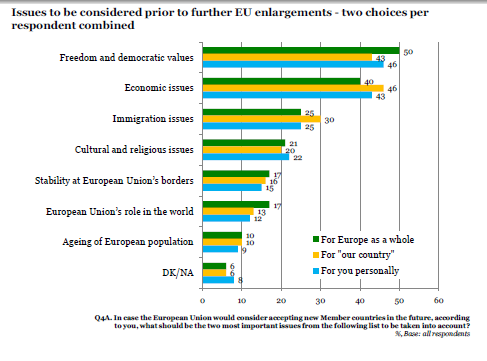
\includegraphics[width=5in]{Material/Umfrage}
\end{figure}
\vspace{-1cm}
{\centering Quelle: Eurobarometer 2009: 20.\footnote{Das Eurobarometer ist eine in regelmäßigen Abständen von der Europäischen Kommission in Auftrag gegebene öffentliche Meinungsumfrage in den Ländern der EU. Dabei werden sowohl immer die gleichen Standardfragen als auch wechselnde Fragen zu unterschiedlichen Themen gestellt.}
  \par
}

In den Mitgliedstaaten der EU wurde folgende Frage gestellt: Falls die EU in der Zukunft über die Aufnahme neuer Mitglieder entscheiden würde, welche zwei Themen (von der vorgegebenen Liste) sollten dabei berücksichtigt werden?

\subsection{Politische Konditionalität im Aufnahmeverfahren}
Um Mitgliedstaat zu werden, muss ein Land den kompletten gemeinschaftlichen Besitzstand der Union (Acquis communautaire) akzeptieren, d.h. in nationales Recht übernehmen. Das gesamte Recht der Europäischen Gemeinschaften und der Europäischen Union wird unter dem Begriff „gemeinschaftlicher Besitzstand“ zusammengefasst. Es handelt sich um rund 15.000 Rechtsakte auf nahezu 100.000 Druckseiten (Stand 2008). Der Acquis communautaire, der seit 1973 in 31 thematische Kapitel eingeteilt war, wurde nach Abschluss der letzten Erweiterungswelle in 35 Kapiteln reorganisiert (vgl. \cite{summa}: 14). \par

\begin{table}[H]
\centering
\setlength\belowcaptionskip{10pt}
\caption{Die Kapitel des Acquis communautaire:}
\begin{tabular}{|c p{7cm}|c p{7cm}|}\hline
1:&Freier Warenverkehr&19:&Beschäftigung und Soziales\\
2:&Freizügigkeit für Arbeitnehmer&20:&Unternehmen und Industrie\\
3:&Niederlassungsrecht und freier Dienstleistungsverkehr&21:&Transeuropäische Netze\\
4:&Freier Kapitalverkehr&22:&Regionalpolitik und Koordinierung der strukturellen Instrumente\\
5:&Öffentliches Auftragswesen&23:&Judikative und Grundrechte\\
6:&Gesellschaftsrecht&24:&Justiz, Freiheit und Sicherheit\\
7:&Rechte am geistigen Eigentum&25:&Wissenschaft und Forschung\\
8:&Wettbewerb&26:&Bildung und Kultur\\
9:&Finanzdienstleistungen&27:&Umwelt\\
10:&Informationsgesellschaft und Medien&28:&Verbraucher- und Gesundheitsschutz\\
11:&Landwirtschaft und ländliche Entwicklung&29:&Zollunion\\
12:&Lebensmittelsicherheit, Tier- und Pflanzenschutzpolitik&30:&Außenbeziehungen\\
13:& Fischerei&31:&Außen-, Sicherheits- und Verteidigungspolitik\\
14:&Verkehr&32:&Finanzkontrolle\\
15:&Energie&33:&Finanz- und Haushaltsvorschriften\\
16:&Steuern&34:&Institutionen\\
17:&Wirtschaft und Währung&35:&Sonstiges \\
18:&Statistik&&\\\hline
\multicolumn{4}{c}{}
\end{tabular}
http://www.europarl.europa.eu/brussels/website/media/modul\_01/Zusatzthemen\\/Pdf/Acquis.pdf  (Aufgerufen: 10.9.2012).
\end{table}
Obwohl es während der Süderweiterung keine auf bestimmte Länder abgestimmten Bedingungskataloge und kein regelmäßiges Monitoring gab, war neben der Übernahme des Acquis communautaire die Demokratie als Staatsmodell ein Aufnahmekriterium (vgl. \cite{pridham07}: 451). Die Assoziierungsvereinbarung mit Griechenland wurde nach dem Staatsstreich der Generäle 1967 eingefroren und der ursprüngliche Aufnahmeantrag Spaniens blieb zunächst unbeantwortet. Dies zeigt, dass die demokratische Verfasstheit schon in dieser Zeit der EU-Erweiterung ein wichtiges, wenn auch implizites Kriterium war. In der Folge ist die EU von der reinen Annahme des Acquis communautaire als Beitrittsbedingung zu weiter gefassten Reform- und Transformationszielen mit zusätzlichen Voraussetzungen übergegangen (vgl. \cite{dimit04}: 8-9).\par
Eine Art politischer Konditionalität wurde erstmals Mitte der 1990er Jahre mit den Europe Agreements eingeführt, die ausgesetzt werden konnten. Gefordert wurde Rechtsstaatlichkeit, Achtung der Menschenrechte, ein Mehrparteiensystem und freie Wahlen (Grabbe zit. in \cite{pridham07}).\par
Seit der Eröffnung einer Beitrittsperspektive für die ehemals kommunistischen Staaten Mittel- und Osteuropas wurden die Kriterien für einen potenziellen Beitritt mit den sogenannten Kopenhagen-Kriterien von 1993 konkreter benannt. Neben ökonomischen Voraussetzungen wird institutionelle Stabilität als eine notwendige Bedingung und Grundlage für demokratische und rechtsstaatliche Ordnung gefordert (vgl. \cite{kreile}: 654). So legte der Rat fest:\par

„Als Voraussetzung für die Mitgliedschaft muss der Beitrittskandidat eine institutionelle Stabilität als Garantie für demokratische und rechtsstaatliche Ordnung, für die Wahrung der Menschenrechte, sowie die Achtung und den Schutz von Minderheiten verwirklicht haben; sie erfordert ferner eine funktionsfähige Marktwirtschaft sowie die Fähigkeit, dem Wettbewerbsdruck und den Marktkräften innerhalb der Union standzuhalten.“ \footnote{Europäischer Rat Kopenhagen, Schlussfolgerungen des Vorsitzes, 21. bis 23. Juni 1993, http://www.consilium.europa.eu/ueDocs/cms\_Data/docs/pressData/de/ec/72924.pdf, S.13 (Aufgerufen: 21.9.2012).}\par

Um die Kriterien von Kopenhagen in konkrete Maßnahmen zu überführen, wurde 1994 das Instrument der „pre-accession strategy“ eingeführt (vgl. \cite{lipsch}). \par

Damit waren die Erweiterungsbedingungen für die Zukunft fixiert. Die EU-Institutionen überprüfen regelmäßig, ob die (potenziellen) Beitrittskandidaten dieses sogenannte politische Kriterium erfüllen. In jährlichen Berichten, die Fortschrittsberichte genannt werden und 1998 erstmals von der Kommission erstellt wurden, überprüft diese, ob Legislative, Exekutive und Verwaltung sowie das Gerichtswesen in den beitrittswilligen Ländern verfassungskonform arbeiten, ob Minderheitenrechte und individuelle Grundrechte geschützt werden und Korruption bekämpft wird (vgl. \cite{brusis09}: 195).
\par
Seitdem kommt der mit den Kopenhagen-Kriterien verbundenen politischen Konditionalität im Rahmen der EU-Erweiterung besondere Bedeutung zu. Ein Wertekatalog gekoppelt an finanzielle Unterstützung im Beitrittsprozess ist das Kennzeichen dieser Entwicklung. Kneuer bezeichnet die Konditionalität des Erweiterungsprozesses als Anreiz-Druck-System, das den attraktiven Anreiz der Mitgliedschaft bietet, aber ebenso Druck im Hinblick auf allgemeine Demokratisierung ausübt und bei demokratischen Defiziten oder Fehlentwicklungen den Druck mit Negativmaßnahmen verstärken kann (vgl. \cite{kneuer07}: 108).\par
Weitere Kriterien bezogen auf die Beitrittsverhandlungen wurden in Madrid anlässlich der Tagung des Europäischen Rates am 14./15. Dezember 1995 formuliert, unter anderem die Forderung nach Verwaltungsreformen in den Kandidatenländern (vgl. \cite{dimit02}). Bezogen auf die Heranführungsstrategie für die Länder Mittel- und Osteuropas forderte der Europäische Rat:
„Diese Strategie muss intensiviert werden, um die Voraussetzungen für eine schrittweise und harmonische Integration dieser Länder zu schaffen, und zwar insbesondere durch die Entwicklung der Marktwirtschaft, die Anpassung der Verwaltungsstrukturen dieser Länder und die Schaffung stabiler wirtschaftlicher und monetärer Rahmenbedingungen“ (\cite{eurrat}).\par
Damit haben die Mitgliedsländer Elemente von „Good Governance“ eingeführt, mit expliziter Erwähnung der Anpassung von Verwaltungsstrukturen (vgl. \cite{sabzei}: 307).\par
Rechtliche und administrative Kapazitäten mussten nun vorhanden sein und wurden als Voraussetzung der Umsetzung des Acquis communautaire gesehen. Damit war die politische Konditionalität als neues Instrument des EU-Erweiterungsprozesses in der letzten Dekade des 20. Jahrhunderts eingeführt worden (vgl. \cite{tomtul}: 380).\par
Die zusätzlichen Bedingungen beziehen sich zum Teil auf Bereiche, in denen die EU selbst nicht über Normenkompetenz oder einheitliche Regelungen verfügt. Zwar gibt es keine direkte Sanktionsmöglichkeit bei der Nichterfüllung der entsprechenden Kriterien, z.B. durch finanzielle Sanktionen. Dennoch ist die „politische Konditionalität“ ein wesentliches neues Element im EU-Erweiterungsprozess. Die Zunahme der Bedeutung von institution building bzw. staatlichen Kapazitäten innerhalb der Erweiterungspolitik der EU wird von Sabel und Zeitlin sogar als Paradigmenwechsel bezeichnet, der sich graduell innerhalb der 1990er Jahre vollzog (vgl. \cite{sabzei}: 307).\par
Der Stellenwert und der Umgang mit der Reform der öffentlichen Verwaltung seitens der EU im Erweiterungsprozess wird im folgenden Kapitel dargestellt.

\subsection{Kompetenz der EU bezüglich der Verwaltung}
\label{subsec:Kompetenz der EU}
Im Bereich der öffentlichen Verwaltung hat die EU keine Regelungskompetenz in den Mitgliedstaaten und keinen direkten Einfluss auf das administrative System ihrer Mitglieder. Alle Mitgliedsländer können die institutionellen Arrangements ihrer öffentlichen Verwaltungen frei wählen, einschließlich des Systems der Ausführung von Staatsaufgaben. Die EU ist bei der Umsetzung des Gemeinschaftsrechts auf die nationalen Verwaltungen angewiesen, ohne Organisationsstrukturen oder Personalstrukturen direkt beeinflussen zu können. Weiterhin existiert innerhalb der EU keine „Blaupause“, die nationale öffentliche Verwaltungen übernehmen können. Es gibt nicht einmal eine Vorstellung eindeutiger „Best Practice“-Beispiele in Bezug auf Strukturen und Verfahrensweisen, obwohl das „White Paper on European Governance“ von 2001 Ausführungsstandards zu beschreiben versucht. „The lack of a clear overarching public administration model and the relatively weak European powers for the imposition of specific changes in domestic administrations might also be considered as a factor for slowing down European Integration“ (\cite{sverdrup}: 44).\par

Das Dilemma der EU hinsichtlich der öffentlichen Verwaltung in den Beitrittskandidaten wird in einem Evaluierungsbericht zur Institutionenentwicklung für die osteuropäischen Beitrittskandidaten deutlich: “Although there are, in many sectors, highly detailed acquis requirements as to what the public administration should deliver, and to what standards, there is of course no acquis on public administration per se” (\cite{omas}: 3). Die Evaluatoren konstatieren, dass die öffentliche Verwaltung nicht Teil des Acquis ist und seitens der EU auch keine Vorgaben für Reformprojekte zur öffentlichen Verwaltung gemacht wurden: “There is no acquis on public administration and there is no evidence that any coordinated attempt has been made by the Commission Services to orientate the PHARE national Public Administration Reform Programmes in any defined direction.” (\cite{omas}: 1). \par

Die Europäische Union hat anlässlich der Erweiterungen 1973, 1980, 1986 und 1995 keine Begutachtung der administrativen Kompetenzen der Aufnahmeländer durchgeführt (vgl. \cite{ziller}: 138). Dennoch sind seit 1997 administrative Fragen im Zusammenhang mit der EU-Erweiterung zunehmend in den Vordergrund gerückt. „Candidate countries have been put under pressure to modernize their administrations, that is, to develop a professional civil service and build institutional capacity to implement and enforce legal norms” (\cite{olsen}). So hat die Präsidentschaft des Europäischen Rates nach ihrem Treffen in Kaeken am 14. und 15. Dezember 2001 angemahnt, dass die Kandidatenländer ihre Anstrengungen fortsetzen müssen, insbesondere um ihre administrativen Kapazitäten auf das geforderte Niveau zu bringen (vgl. \cite{olsen}). Hintergrund dieser Forderung ist vor allem die Notwendigkeit, nationale Verwaltungsstrukturen zu entwickeln, die für die Interaktion mit der EU verantwortlich sind für die Verhandlungen mit Brüssel und die Umsetzung des Acquis.

\subsection{Das Konzept des Europäischen Verwaltungsraumes}
\label{subsec:Verwaltungsraum}
Nachdem nun deutlich wurde, dass es keinen konkreten Acquis zur Ausgestaltung der öffentlichen Verwaltung gibt, stellt sich die Frage, ob es möglicherweise durch die Zunahme supranational zustande gekommener Entscheidungsprozesse zu einer Europäisierung im Verwaltungshandeln kommt. Einerseits hat die EU keinen direkten Einfluss auf die verwaltungsmäßige Umsetzung von Gemeinschaftsrecht. Andererseits erscheint eine Art Blaupause für Strukturen einer europäisch orientierten Verwaltung sinnvoll angesichts der möglichen Aufnahme von Ländern mit schwacher demokratischer Staatstradition (z.B. Bosnien-Herzegowina, Albanien). Vor allem die Organisation für Ökonomische Zusammenarbeit und Entwicklung (OECD) mit ihrem SIGMA-Programm (Support for Improvement in Governance and Management) war seit 1998 maßgeblich an der Entwicklung eines Konzeptes zu einem europäischen Verwaltungsraum (European Administrative Space) beteiligt. SIGMA kam im Rahmen einer Studie zu der Auffassung, dass die strikte Auslegung von Artikel 39 Absatz 4 EG-Vertrag und des Begriffs der „Öffentlichen Verwaltung“ durch den EuGH zur Schaffung eines Verwaltungsraumes in den Mitgliedstaaten führen wird. Die European Group of Public Administration (EGPA) des Internationalen Instituts für Verwaltungswissenschaften richtete 2002 eine Tagung aus zum Thema: „ The European Administrative Space: Governance in Diversity“ (\cite{mangenot}: 13).\par
In Anbetracht der unterschiedlichen Traditionen der öffentlichen Verwaltung in Europa gibt es Stimmen, die vor der Ausrufung eines gemeinsamen europäischen Rahmens für den öffentlichen Sektor warnen (vgl. \cite{olsen}). Gründe für diese angemahnte Vorsicht sind unter anderem nach wie vor nationale Weichenstellungen. Die EU hat gerade erst angefangen, die Reform der öffentlichen Verwaltung als eigenständiges Politikfeld zu sehen (vgl. \cite{schmar}). Weiterhin hat die EU kein starkes Rollenmodell im Bereich Public Management für die Mitgliedstaaten geschaffen und die zentrale Verwaltung der EU erscheint als ein Patchwork einzelner unterschiedlicher nationaler Traditionen. Dennoch kann von einem Trend hin zu einem spezifischen europäischen Ansatz im Bereich öffentlicher Verwaltung ausgegangen werden. Dies kann auch damit erklärt werden, dass es in den EU-Mitgliedsländern eine gemeinsame Idee von Staat, Souveränität und Demokratie gibt, zumindest im Vergleich mit anderen Kontinenten. Insbesondere der Acquis communautaire, der zentrale Teil der EU-Gesetzgebung, stellt eine Basis dar für gemeinsame administrative Standards und Regeln, die Eingang finden in das System der nationalen öffentlichen Verwaltung (vgl. \cite{raarut}: 31). Weiterhin entspricht das Konzept eines Europäischen Verwaltungsraumes der Forderung von Wirtschaftsakteuren nach einheitlichen Wettbewerbsbedingungen und nach administrativer Kooperation über Ländergrenzen hinweg (vgl. \cite{bogjan}: 245). \par
Gemeinsame Grundwerte und -prinzipien der europäischen öffentlichen Verwaltung haben zunehmend zu Konvergenz zwischen nationalen Verwaltungen geführt. „The European Administrative Space (EAS) represents an evolving process of increasing convergence between national administrative legal orders and administrative practices of member states. The EAS concerns basic institutional arrangements, processes, common administrative standards, civil service values and administrative culture. It is difficult to speak of a European model of Public Administration, but the EAS, albeit a metaphor, signifies a convergence and states the basic values of public administration as a practice and profession in Europe” (\cite{oecd99}: 15). \par
Mit der Stärkung und Erweiterung der EU sind im Hinblick auf die administrative Konvergenz viele Hoffnungen verbunden. So wird von einer Homogenisierung der administrativen Kapazitäten ausgegangen, unter Einbezug nationaler und kultureller Besonderheiten. Dabei geht es nicht um eine „Gleichschaltung“ der administrativen Systeme, sondern um eine Angleichung der Serviceerbringung hinsichtlich Qualität und Effizienz im Sinne eines Public Service Standards, so eine Sichtweise (vgl. \cite{dorta}: 8f.). Allerdings gibt es auch Stimmen, die auf die Bedeutung der nationalen Verwaltungstraditionen hinweisen. Selbst eindeutig auf europäischen Regelungen basierende Veränderungsprozesse der nationalen Verwaltungen sind nach dieser Perspektive entscheidend durch den nationalen Kontext geprägt (vgl. \cite{herit}).\par
Auf einer praktischen Ebene kann man bei dem ‚European Public Administration Network' (EUPAN)\footnote{http://www.eupan.eu/en/content/show/\&tid=188 (Aufgerufen 15.10.2012).}, in dem Minister und Generaldirektoren des öffentlichen Dienstes vertreten sind, von einer Europäisierung durch Verwaltungskooperation sprechen. In dem Netzwerk war von Anfang an auch die Europäische Kommission mit dem für die Verwaltungsreform zuständigen Kommissar der Generaldirektion Verwaltung und Personal (ADMIN) vertreten; dennoch steht EUPAN außerhalb des förmlichen Rahmens der Gemeinschaft. EUPAN dient als Netzwerk und fördert durch das Zusammentreffen von nationalen Beamten den Austausch über Ländergrenzen hinweg (vgl. \cite{mangenot}: 49).\par
Eine andere (europäische) Initiative, das ‚Common Assessment Framework’ (CAF), mit dem Ziel, Exzellenz in der europäischen öffentlichen Verwaltung zu fördern, soll hier ebenfalls erwähnt werden. Das CAF wurde im Anschluss an das Ministertreffen vom November 1998 entwickelt, als die Schaffung eines „Europäischen Qualitätspreises“ auf Grundlage von Leistungsindikatoren vorgeschlagen wurde. Das im Mai 2000 in Lissabon auf der ersten europäischen Qualitätskonferenz vorgestellte CAF basiert auf Modellen der Europäischen Stiftung für Qualitätsmanagement (European Foundation for Quality Management) und ist ein Instrument der Selbstbewertung von öffentlichen Verwaltungen (vgl. \cite{mangenot}: 52).\par
Im Lissabonner Vertrag, der 2009 in Kraft trat, wurde erstmals eine Verwaltungszusammenarbeit direkt erwähnt. Mit dem Vertrag von Lissabon wurden die beiden „Gründungsverträge“ der EU, d.h. der Vertrag über die Europäische Union (EUV) und der Vertrag zur Gründung der Europäischen Gemeinschaft (EGV), der in Vertrag über die Arbeitsweise der Europäischen Gemeinschaft (AEUV) umbenannt wurde, grundlegend und umfassend geändert. Der eigentliche Lissabon-Vertrag, enthält die jeweiligen Änderungen am EUV und am AEUV (ex-EGV). Dies betrifft auch Artikel 176 des AEUV, in dessen veränderter Version unter Artikel 176d erstmals ausdrücklich eine Verwaltungszusammenarbeit genannt wird: „Die Union kann die Mitgliedstaaten in ihren Bemühungen um eine Verbesserung der Fähigkeit ihrer Verwaltung zur Durchführung des Unionsrechts unterstützen. Dies kann insbesondere die Erleichterung des Austauschs von Informationen und von Beamten sowie die Unterstützung von Aus- und Weiterbildungsprogrammen beinhalten. Die Mitgliedstaaten müssen diese Unterstützung nicht in Anspruch nehmen. Das Europäische Parlament und der Rat erlassen die erforderlichen Maßnahmen unter Ausschluss jeglicher Harmonisierung der Rechtsvorschriften der Mitgliedstaaten durch Verordnungen gemäß dem ordentlichen Gesetzgebungsverfahren“ (\cite{verLis}: C306/90). \par
Ein weiterer Versuch, das Thema Verwaltungsmodernisierung im Erweiterungsprozess zu operationalisieren, stellt die sogenannte PAR checklist der Generaldirektion Verwaltung (DG ADMIN) dar. 

{\bf “PAR checklist”}
\label{sub:par checklist}
\begin{enumerate}
\item PAR framework 
\begin{itemize} \itemsep1pt \parskip0pt \parsep0pt
\item Political will
\item Authority in charge with the coordination of the PAR
\item Comprehensive reform programme: reform strategy/action plan established + implemented after consultation with different stakeholders
\item Acceptance of the reform at all central/local/regional levels
\item Legal background on PA organization and administrative procedures endorsed and implemented
\item Integration of principles of a sound PA derived from the Community law
\end{itemize}
\item Civil service quality
\begin{itemize} \itemsep1pt \parskip0pt \parsep0pt
\item Structure in charge with civil service management
\item Legal acts endorsed and implemented (civil service act + secondary legislation – rights and obligations, ethics and integrity, merit + equal chances + transparency based recruitment, fair appraisal and promotion systems, appeals procedures, basic salary systems formalised + transparent bonus allocation policy, training, pension systems …)
\item HR instruments (CAF, competency frameworks, personal benchmarks, career guidance schemes, fast track…etc.)
\end{itemize}
\item Anti-corruption policy
\begin{itemize} \itemsep1pt \parskip0pt \parsep0pt
\item Political will to fight against corruption
\item Establishment/existence of independent anti-corruption bodies
\item Instruments to prevent, detect and penalise corruption (effective legal framework, anti-corruption strategies or laws, watchdog agencies, codes of conduct, penal laws, regulation of conflict of interest and incompatibilities, rules to ensure transparency and accountability in financial management, disciplinary procedures…)
\item Facultative requirements: ethic counselors, exchange of best practices, awareness campaigns, whistleblowers procedures…
\end{itemize}
\item Transparency and citizen orientation 
\begin{itemize} \itemsep1pt \parskip0pt \parsep0pt
\item Body/ies representing public interest (ombudsman.…)
\item Legal acts (law on free access to public information, law on treating citizens’ complaints, provisions on regular consultation of citizens…) 
\item Transparency instruments (public events, citizens’ charters, e-government instruments, regular consultation of public opinion, one-stop shops, information centers…)”
(\cite{butiu}: 13)
\end{itemize}
\end{enumerate}

Diese checklist wurde im Entwurf diskutiert und die Idee von einzelnen Akteuren in Brüssel, Paris sowie in den Beitrittsländern selbst aufgenommen. Eine verbindliche Richtschnur ist damit allerdings nie verbunden worden. Dies wohl auch zum Teil aus Sorge der Mitgliedsländer, dass damit eine Einmischung in die Strukturen ihrer eigenen öffentlichen Verwaltungen gerechtfertigt werden könnte. \par
Die Ausgestaltung der öffentlichen Verwaltung liegt im Ermessen der EU-Mit\-glieds\-län\-der und ist eng verbunden mit der historischen Entwicklung der Verwaltung. In Europa gibt es unterschiedliche Verwaltungstraditionen und eine Vereinheitlichung erscheint aus diesem Grund schwer möglich und nicht gewünscht. Dennoch ist die Bedingung der Übernahme des Acquis communautaire bei einer EU-Mitgliedschaft eine immense Herausforderung insbesondere für die öffentlichen Verwaltungen der Beitrittsländer. Mit zunehmendem Einfluss der EU auf Binnenprozesse gewinnen supranationale Ansätze auch in Bezug auf die Ausgestaltung bzw. Modernisierung der nationalen öffentlichen Verwaltungen Gewicht. Stichworte dazu sind European Administrative Space, Common Assessment Framework und EU PAR checklist zu Verwaltungsmodernisierung. Auch der Lissaboner Vertrag von 2009 erwähnt zum ersten Mal die Verwaltungskooperation. Dennoch sind alle diese Ansätze nur punktuell und haben keinen verbindlichen Charakter.\par
Dass sich aus dieser fehlenden Verbindlichkeit zum Thema Verwaltungsentwicklung und -modernisierung Probleme für die EU bei der Erweiterung ergeben, zeigt ein Blick auf die letzte Erweiterungswelle nach Osteuropa. Einen Überblick über die Erfahrungen zur Verwaltungsentwicklung in diesen Ländern bietet der folgende Abschnitt.

\subsection{Erfahrungen zur Verwaltungsentwicklung in den Staaten Osteuropas}
\label{subsec:Verwaltungsentwicklung}
Die vorliegende Literatur zu den Erfahrungen der EU-Erweiterung in den Ländern Osteuropas, die 2004/7 beitraten, wurde im Hinblick auf den Stellenwert der Reform der öffentlichen Verwaltung im Erweiterungsprozess gesichtet. Da es sich bei den Ländern der Osterweiterung ebenfalls um vormals zentralistisch organisierte Staaten handelte, können möglicherweise übertragbare Erkenntnisse für die anstehende Südosterweiterung gewonnen werden. \par

Beitrittsvereinbarungen, die so genannten Europe Agreements, wurden von der EU mit den osteuropäischen Beitrittskandidaten zwischen 1991 und 1996 unterzeichnet und die Länder stellten zwischen 1994 und 1996 die offiziellen Aufnahmeanträge. In den darauffolgenden Jahren, in denen die Heranführung der Länder an die EU seitens der EU unterstützt wurde, führte der Wunsch nach schneller Aufnahme oft zu vordergründigen Reformen „The overarching goal of wanting to join the EU as quickly as possible, however, dominated the governments’ behaviour and more strategic work on policy priorities seldom got significant early attention“ (\cite{summa}: 10).\par
In den früher zentralistisch regierten Ländern des Ostblocks waren die Dezentralisierung und die Etablierung demokratischer lokaler Regierungsstrukturen nach dem Systemwechsel vorrangige Ziele. Mit der Dezentralisierung eng verknüpft ist auch die effektive Erfüllung öffentlicher Aufgaben. Ein wesentliches Ziel in diesem Zusammenhang ist die Trennung der zentralen und der lokalen Verwaltung bei der Aufgabenerfüllung, im Gegensatz zu der vormals direkten Unterstellung der lokalen Verwaltung unter die Zentralgewalt. Dezentralisierung und Reform der öffentlichen Verwaltung gingen und gehen also in den betroffenen Ländern Hand in Hand. Der nächste Schritt ist in der Regel die Reform des civil service, weg von politischer Loyalität hin zu neutralen Mitarbeitern, die an Recht und Gesetz gebunden sind. Dabei sind veränderte Gesetze zentral, aber nur der erste Schritt. Eine entsprechende Implementierung mit klaren Karriereschritten und Training der öffentlich Bediensteten muss folgen. Für diese umfassenden Reformschritte stellen internationale Institutionen wie die Weltbank, EBRD, UNDP, bilaterale Institutionen und auch die EU Mittel zur Verfügung.\par
Die Erfahrungen der Länder der östlichen EU-Erweiterung zeigen, dass die Veränderungen auf allen oben erwähnten Ebenen gleichzeitig angegangen werden müssen. Dabei gab es in den Ländern durchaus Unterschiede in der Entwicklung. In Ungarn und Polen wurden politische und institutionelle Veränderungen anfänglich in großem Tempo vorgenommen, danach jedoch dauerte der Prozess der Umsetzung fast eine Dekade. In Bulgarien und Lettland führten die revolutionären Ereignisse zu Unabhängigkeit und neuer Verfassung, doch die Reform des öffentlichen Sektors wurde vernachlässigt. Nach mehreren Jahren der Stagnation wurden die Gebietsreform und die Modernisierung der lokalen Verwaltungen erst Ende der 90er Jahre begonnen. In einer dritten Gruppe von Ländern (vor allem Kroatien und Slowakei) begannen die wesentlichen Strukturreformen nicht nur spät, sondern in den ersten zehn Jahren der Transformation wurden keine wesentlichen Reformen durchgeführt (vgl. \cite{petzen}: 19).  \par

Studien zur EU-Osterweiterung zeigen, dass je stärker die nationalen administrativen Strukturen und Traditionen waren, desto mehr Resistenz gegenüber Anpassungsdruck im Zusammenhang mit der EU-Erweiterung entstand (vgl. \cite{knill01, goetz01b}). Im Wesentlichen hat in diesen Fällen Policy-Transfer stattgefunden, der innerhalb der bestehenden Strukturen umgesetzt werden konnte, ohne die Verwaltungsstrukturen entscheidend zu beeinflussen. Ein einheitliches Modell der öffentlichen Verwaltung ist nicht entstanden. Eine Studie zu Ungarn fasst zusammen: „Of course, the national administrative culture is not untouchable or completely intact towards external impacts. But it is also true that it has considerable ability to make processes slow or resist new behavioural patterns and untested ideas and practices” (\cite{szente}: 59). Zu einer insgesamt kritischen Einschätzung der externen Unterstützungsmaßnahmen und ihrer Auswirkungen im Rahmen der Osterweiterung der EU kommt Coombes, der von häufig unklaren oder gar widersprüchlichen Zielvorstellungen der Programme spricht. Oft würden diese nicht der Realität in den Empfängerländern gerecht. Dennoch käme es durch die Projekte zu sogenannten „trickle-down“-Effekten. In diesem Sinne ist der Wissenstransfer, auch durch EU-Förderprogramme bei aller angebrachten Kritik positiv zu bewerten: „…there is usually some, more or less hidden, indirect benefit of knowledge transfer and learning – albeit in aspects not specifically projected by donors – which enhance the value of human capital in the recipient countries” (\cite{coombes}: 6). \par

In eine ähnliche Richtung geht Brusis’ Beobachtung, „dass sich im Bereich der Verwaltungsreform viele vage und doppeldeutige EU-Signale beobachten lassen, da sich die demokratische und administrative Konditionalität überlagerten“ (\cite{brusis09}: 99). Neben Fällen, in denen sich Regierungen auf EU-Erwartungen berufen haben, um eigene Reformprojekte zu realisieren, gibt es auch die so genannte „Potemkinsche Harmonisierung“, bei der formale Strukturen aufgebaut wurden, um den Forderungen der EU nachzukommen, diese aber wenig oder keinen Einfluss auf die nationalen ‚outcomes’ hatten (vgl. \cite{schsed05a}: 17). Obwohl einige sektorale Ansätze sich mit der Reform der öffentlichen Verwaltung beschäftigten, gab es im Zusammenhang mit der Ost-Erweiterung in dieser Hinsicht keine systematische Vorgehensweise seitens der EU. „There were no systematic attempts at benchmarking key public administration reform objectives, no formal mechanism for disseminating good or best practices, and donor coordination fell short of expectations” (\cite{summa}: 21). Eine andere Sichtweise geht davon aus, dass die EU die falschen Anreize gegeben habe mit ihrer Konzentration auf die Berichterstattung zum Fortschritt der Übernahme des Acquis. „The detailed requirements of the Commission in the field of governance and the related conditionality created a relationship where the EC became the sole principal (instead of domestic publics or their representatives) and the government its agent. Reforms were not driven by impact evaluations, but by the need to satisfy the pressing bureaucratic reporting needs for the EC regular monitoring reports. ‘One-off special efforts” to reach certain EU deadlines and ‘islands of excellence’ units …prevailed while sound, system-building administrative reform was neglected” (\cite{mungiu}: 17). \par

Verheijen identifiziert im Hinblick auf die Verwaltungsentwicklung der Länder der letzten Erweiterungswelle ein „mixed picture of overall setbacks“. Zentrale Elemente der öffentlichen Verwaltung werden weiterhin als problematisch eingestuft, allen voran der civil service. So konstatiert er eine große Bandbreite unterschiedlicher Reformen, die nicht auf einem allgemein anerkannten Modell beruhen. Auch die weiterhin zum Teil starke Politisierung und damit sich häufig ändernde Reformorientierungen in den Ländern der letzten Erweiterungswelle tragen zu dem Bild bei. „The lack of underlying consensus has been clearly visible in the merry-go-round of reforms in the civil service in both Poland and Hungary” (\cite{verheijen06}: 48). \par

In einer Studie zur Reform des civil service in den Ländern der östlichen EU"=Erweiterung werden als zentrale Elemente strukturelle Probleme in nach-kom\-mu\-ni\-sti\-schen Verwaltungen angeführt: 
\begin{itemize} \itemsep1pt \parskip0pt \parsep0pt
\item Fast vollständige Politisierung der öffentlichen Verwaltung. Die Vorbereitung von policies und Gesetzen sowie die Umsetzung der policies waren mit großem politischem Einfluss der Zentralregierung und der Regierungspartei verbunden. 
\item Ethische Prinzipien wie „Neutralität“ und „Unbestechlichkeit“ wurden oft aufgrund der starken Politisierung gebrochen.
\item Fehlende Mobilität im civil service. Darüber hinaus waren Karrierechancen und Beförderung eng mit der Anpassung an politische Präferenzen verbunden.
\item Ein hoher Grad an Fragmentierung von Verantwortlichkeit in der Personalpolitik. 
\item In den meisten Fällen gab es keine Stelle, die für Rekrutierung zuständig war, sondern die entsprechenden Minister hatten diese Kompetenz.
\item Schlechtes Image des Beamtentums und schlechte Verdienstmöglichkeiten
(vgl. \cite{bosdem}: 3). 
\end{itemize}

Als problematisch benennt Verheijen die Umsetzung nicht sinnvoll zugeschnittener Reformmodelle, insbesondere wenn die Angst bestand, dass die EU nicht ausreichende administrative Kapazität als Grund für einen Aufschub der EU-Mitgliedschaft anführen könnte. Besonders in der Slowakei als „Spätreformierer“ dürfte dies zugetroffen haben. Wesentliche Gründe für Rückschritte in der administrativen Reformagenda waren Uneinigkeit über die Richtung der Reformen (Polen, Estland, evtl. Ungarn). Auch ein Mangel an Interesse unter Politikern an einer Reform der öffentlichen Verwaltung wirkte sich negativ aus, besonders in der Tschechischen Republik. Hier ging man davon aus, ökonomische und politische Erfolge würden verhindern, dass die EU im Hinblick auf Verwaltungsreformen Druck ausüben könnte (vgl. \cite{verheijen06}: 43). \par

In Lettland und Litauen waren nach anfänglichem Experimentieren mit Verwaltungsreformen in den 1990er Jahren ab 2000 drei wesentliche Voraussetzungen für erfolgreiche Reformen erfüllt. Es gab:
\begin{enumerate} \itemsep1pt \parskip0pt \parsep0pt
\item  eine weitgehende Übereinstimmung über die Richtung der Reformen,
\item eine angemessen große Zahl reformorientierter Entscheidungsträger mit entsprechender Motivation, 
\item eine relative kleine Gruppe von Verwaltungsreformern, die das Vertrauen und die Unterstützung wechselnder politischer Gruppen sichern konnten (vgl.  \cite{verheijen06}: 44).
\end{enumerate}

Die Erfahrung der EU-Erweiterung mit der Aufnahme Bulgariens und Rumäniens 2007 als letzte Länder der Osterweiterung macht deutlich, dass Konditionalität in diesen beiden Fällen strikter angewendet wurde als bei früheren Aufnahmen. Auch die administrative Kapazität, als wichtige Voraussetzung für die Übernahme des Acquis communautaire, gelangte stärker in den Blick. Es wurden Monitoring-Maßnahmen eingeführt und bisher nicht bekannte Verzögerungsklauseln aufgenommen. Diese Verzögerungsklauseln für Bulgarien und Rumänien beinhalteten die Möglichkeit einer Verschiebung der Aufnahme um ein Jahr, fanden aber keine Anwendung (vgl. \cite{phinnemore}: 2). Stattdessen entwickelte die EU-Kommission einen „Mechanism for Cooperation and Verification of Progress in the areas of judicial reform and the fight against corruption, money-laundering and organized crime” (CVM). In diesem Rahmen mussten die beiden Länder Bulgarien und Rumänien über speziell festgelegte Eckpunkte regelmäßig an die EU-Kommission berichten (vgl. \cite{summa}: 24). 
\par
Einerseits zeigen Erfahrungen in den Ländern Osteuropas, dass externe Anreize und finanzielle Unterstützung durchaus zu einer Modernisierung des Verwaltungsapparates führen können. Andererseits wird auch deutlich, dass der Druck der EU nicht ausreichte, um erfolgreiche Verwaltungsreformen auf den Weg zu bringen, da:
\begin{itemize} \itemsep1pt \parskip0pt \parsep0pt
\item der Druck der EU hinsichtlich der administrativen Kapazität nicht effektiv ist, 
\item der Zeitrahmen bis zur Aufnahme nicht ausreichend war für eine effektive und umfassende Umsetzung einer Verwaltungsreform (vgl. \cite{verheijen06}: 44).
\end{itemize}
Angesichts des nur indirekten Mandates der EU, Verwaltungsreformen einzufordern, ist der überwiegend negative Befund für die letzte Welle der Beitrittsländer hinsichtlich ihrer administrativen Kapazitäten nicht überraschend.\par
Auch nach der Aufnahme in die EU bleibt die administrative Kapazität der Länder Osteuropas problematisch. Obwohl es einige positive Beispiele in bestimmten Bereichen gibt, die unter großem Ressourceneinsatz zustande kamen, ist das übergeordnete Bild ernüchternd. Ein spezifisches Problem ergibt sich daraus, dass die Länder oft nicht in der Lage waren, die EU-Strukturfonds angemessen zu managen. Besonders die geringe Absorptionsquote der EU-Gelder im Zeitraum 2004 bis 2006 gab Anlass zur Sorge. Am Beispiel von Ungarn und Polen, die ungeachtet ihres Status als „best pupils of enlargement“ nicht das gesamte ihnen zur Verfügung stehende PHARE-Budget nutzten, konstatierte die EU-Kommission, „the lack of administrative capacity and political will as well as the poor involvement of civil society in shaping the reforms“ (\cite{tulmets06}: 6).\par
In einer Untersuchung zu den neuen EU-Mitgliedsländern stellt Verheijen eine hohe Korrelation fest zwischen Ländern, die ihre öffentliche Verwaltung substanziell verbesserten, und dem allgemeinen Funktionieren innerhalb der EU. Solche Staaten, wie Lettland, Litauen und mit etwas Abstand die Slowakei, haben in einer Studie mit performance-indicators für die öffentliche Verwaltung der Weltbank wesentlich besser abgeschnitten als Länder mit geringerer Reformorientierung, wie Polen und Ungarn. „While the former states (Lettland, Litauen, Slowakei C.V.) made progress both on the introduction of performance-based public management systems and, to a lesser degree, on civil service reform, virtually no progress has been made on these aspects of administrative governance in the latter (Polen, Ungarn C.V.)” (\cite{verheijen09}: 4).\par
In einem internen Diskussionspapier der EU\footnote{Das Papier wurde der Verfasserin dieser Arbeit vom Autor zur Verfügung gestellt.} werden weitere Gedanken zur relativen Erfolglosigkeit der Unterstützung von Verwaltungsreformen im Zuge der EU-Osterweiterung entwickelt. Als problematisch benannt werden Geberdominanz, fehlender politischer Wille der nationalen Akteure und geringe Absorption der bereitgestellten Mittel: „Mainstream evidence shows that in the past a considerable part of the support for horizontal public administration reform largely failed as it was supply-driven without sufficient consideration of the demand-side issues of political commitment, change management and absorption capacity” (\cite{apelb07}: 2). \par
Den begrenzten Effekt der EU-Erweiterung auf die öffentliche Verwaltung in den neuen Mitgliedsländern der EU erklären Lippert und Umbach mit dem Umstand, dass Verwaltungsmodernisierung nicht Teil des Acquis communautaire ist und somit keine starken Interventionen seitens der EU stattfinden können. „Die Europäische Union, die in ihrer Erweiterungspolitik frühzeitig der Normalisierungsthese im Hinblick auf die Entwicklung der Verwaltung in den Ländern Mittel- und Osteuropas anhing, hat sich zunehmend auf die Rolle eines Wächters und nachfrageorientierten Assistenten und Vermittlers von Lösungsangeboten aus den EU-15 beschränkt, statt die Rolle einer aktiven Entscheidungsinstanz oder eines Exporteurs eines idealtypischen EU-kompatiblen Verwaltungsmodells zu beanspruchen“ (\cite{lipumb04}: 73).
\par
Zu ähnlichen Ergebnissen kommt die Analyse eines Experten zur Reform der öffentlichen Verwaltung innerhalb der EU-Kommission: „Enlargement is rightly largely seen as a ‘success story’ but the benefits which citizens and enterprises could have enjoyed from their countries joining the EU would probably have been greater if the support to horizontal PAR had been more effective, more timely, more coordinated and more strategic” (\cite{apelb09}: 5).\par
Verbindet man die theoretischen Ansätze zur EU-Erweiterung mit den praktischen Erfahrungen, so zeigt sich, dass die Praxis der EU in Bezug auf die Verwaltungsentwicklung im Erweiterungsprozess vor einem Dilemma steht. Einerseits wird seitens der EU von politischer Konditionalität gesprochen. Nur mit entsprechender administrativer Kapazität ist die Übernahme des Acquis communautaire umzusetzen. Andererseits hat die EU kein Modell der öffentlichen Verwaltung, an dem sich die Beitrittsländer orientieren könnten. Alle Versuche in diese Richtung mündeten bisher nicht in verbindlichen Modellen, was auch mit der Hoheit der einzelnen Länder in der Verwaltungsgestaltung erklärbar ist. Folgerichtig ist die Ausgestaltung der Verwaltung oder die Verwaltungsmodernisierung kein Kapitel des Acquis. Um weiteres Licht in diese von der Forschung bisher weitgehend unausgeleuchteten Zusammenhänge zu bringen, soll ein Blick auf die Geschichte der Beziehungen der EU zu den Ländern des Westlichen Balkans bei der weiteren Spurensuche helfen.

\section{Institutionelle Beziehungen der EU zu Südosteuropa}
Anders als zu den Ländern der Osterweiterung, die in der Zeit des Kalten Krieges unter dem Einfluss der Sowjetunion standen und kaum Beziehungen zur EU pflegten, kann die EU auf schon frühe Beziehungen zu Jugoslawien zurückblicken. Finanzielle Unterstützung für Jugoslawien in Form von direkten Hilfen durch die Europäische Wirtschaftsgemeinschaft (EWG) wurde ab Anfang der 1960er Jahre gewährt. Wirtschaftliche Beziehungen der EWG zu Südosteuropa gehen zurück in die 1970er Jahre, als Jugoslawien ein Handelsabkommen mit der EWG für eine schrittweise Handelsliberalisierung und eingeschränkte Kreditmöglichkeiten schloss. Weiterhin ermöglichten entsprechende Abkommen, dass ab den 1970er Jahren sogenannte Gastarbeiter in den Ländern der EWG arbeiten konnten (vgl. \cite{weithmann}: 447). Dennoch führten die Entwicklungen der 1990er Jahre im ehemaligen Jugoslawien mit einem zerfallenden föderalen Staat und schneller bilateraler Anerkennung von Teilstaaten als eigenständigen Ländern (Kroatien und Slowenien) sowie Kriege in der Region zunächst zu einer Art Bewegungsunfähigkeit der EU in Bezug auf Südosteuropa (vgl. \cite{inotai}: 21).\par
Während die osteuropäischen Staaten in den 1990er Jahren mit verschiedenen Mechanismen auf eine Integration in die EU vorbereitet wurden, spitzten sich in dieser Zeit auf dem Westbalkan ethnische Konflikte zu, Kriege wurden ausgetragen und Staaten zerfielen. Das Ergebnis waren neue schwache Staaten, zum Teil unter internationaler Verwaltung. Dennoch blieb die EU-Orientierung ein Hauptziel praktisch aller Regierungen der Länder des westlichen Balkans. Und auch die internationale Staatengemeinschaft hatte ein Interesse daran, den Westbalkan in den europäischen Kontext einzubinden. Ein „Regionalkonzept“ diente als Rahmen für die Entwicklung der Beziehungen der EU zu den Ländern der Region. Die Ziele dieses Regionalkonzepts von 1996 waren die Unterstützung der Friedensabkommen von Dayton/Paris sowie die Schaffung einer Zone politischer Stabilität.\par
Der Stabilitätspakt für Südosteuropa (1999) zielte auf eine Ablösung der bisherigen Politik der Krisenintervention in der Region durch eine umfassende und langfristige Konfliktpräventionsstrategie. Der Stabilitätspakt bestand aus einer politischen Verpflichtungserklärung und einer Rahmenvereinbarung zur internationalen Kooperation in Südosteuropa zwischen mehr als 40 Staaten, Organisationen und regionalen Zusammenschlüssen. Am Stabilitätspakt waren u.a. die Vereinten Nationen, die OSZE, die Europäische Kommission, alle EU-Mitgliedsländer, die Länder Südosteuropas aber auch die USA, Japan, Kanada und Russland beteiligt. Ziel war es, die Länder in Südosteuropa in der Demokratisierung und ökonomischen Entwicklung zu unterstützen.\footnote{http://www.stabilitypact.org/about/default.asp (Aufgerufen: 1.9.2012).} Ein Sonderkoordinator führte den Vorsitz beim Regionaltisch, dem wichtigsten politischen Instrument des Stabilitätspaktes. Diesem untergeordnet waren drei Arbeitstische:
\begin{enumerate}[label=Tisch {\Roman*}:,align=left,  leftmargin=*]
\item Demokratisierung und Menschenrechte
\item Wirtschaftlicher Wiederaufbau, Zusammenarbeit und Entwicklung
\item Sicherheitsfragen
\end{enumerate}
Innerhalb des Arbeitstisches I beschäftigte sich eine Arbeitsgruppe (Task Force) „Good Governance“ unter Vorsitz des Europarats vorrangig mit der Entwicklung der Kommunalverwaltungen, mit der Einsetzung von Ombudspersonen sowie der Reform der öffentlichen Verwaltung (vgl. \cite{calic01}: 9). Die Bedeutung des Stabilitätspaktes nahm in dem Maß, in dem die EU ihre Südosteuropapolitik weiterentwickelte, ab.
\par
Im Rahmen des Stabilitätspaktes legte die Europäsche Union 1999 einen Sta\-bi\-li\-sie\-rungs- und As\-so\-zi\-ie\-rungs\-pro\-zess (SAP) für Südosteuropa auf. Dieser hatte folgende Ziele für die Region:
\begin{itemize} \itemsep1pt \parskip0pt \parsep0pt
\item Konzipierung von Stabilisierungs- und Assoziierungsabkommen mit der Aussicht auf einen
Beitritt zur Europäischen Union, wenn die Kopenhagener Kriterien erfüllt sind;
\item Ausbau der wirtschaftlichen und handelspolitischen Beziehungen zu dieser Region sowie innerhalb der Region;
\item Erhöhung der wirtschaftlichen und finanziellen Hilfe;
\item Unterstützung der Demokratisierung, der Zivilgesellschaft und des Aufbaus von Institutionen;
\item Zusammenarbeit im Bereich Justiz und Inneres;
\item Intensivierung des politischen Dialogs (vgl. \cite{marwedel}: 9).
\end{itemize}

Ausgangspunkt einer erstmals konkreteren EU-Perspektive für die Staaten des Westbalkans war die Tagung des Europäischen Rates im Juni 2000 in Feira: „Ziel ist, die [westlichen Balkanstaaten] im Wege des Stabilisierungs- und Assoziierungsprozesses, des politischen Dialogs, der Liberalisierung des Handels und der Zusammenarbeit im Bereich Justiz und Inneres so weit wie möglich in den Strom der allgemeinen politischen und wirtschaftlichen Entwicklung Europas einzubeziehen. Alle betroffenen Länder sind potenzielle Bewerber für den Beitritt zur EU“ (\cite{euko05}: 3). Im November 2000 wurde in Zagreb der SAP-Prozess offiziell eingerichtet und drei wesentliche Instrumente eingeführt: 1) bilaterale begünstigte Handelsabkommen, 2) das CARDS-\footnote{„Community Assistance for Reconstruction, Democratization and Stabilization“ (siehe auch Abschnitt \ref{subsec:Kompetenz der EU})}Programm zur finanziellen Unterstützung ausgewählter Projekte und 3) die Unterzeichnung von Stabilisierungs- und Assoziierungsabkommen bei Erfüllen bestimmter Kriterien. Die erfolgreiche Umsetzung des SAP eröffnete den Weg zu einem Stabilisierungs- und Assoziierungsabkommen (SAA) und darauf aufbauend zu der Beantragung der EU-Mitgliedschaft (vgl. \cite{inotai}: 25). \par
Bestätigt wurde die Beitrittsperspektive der Länder des Westlichen Balkans im Juni 2003 in Thessaloniki mit der „Agenda von Thessaloniki für die westlichen Balkanstaaten: Auf dem Weg zur Europäischen Integration“. Die nächste Stufe der institutionellen Kooperation zwischen der EU und den Ländern des Westbalkans waren Stabilisierungs- und Assoziierungsabkommen. Diese Abkommen haben eine ähnliche Funktion wie die Europäischen Partnerschaften mit den osteuropäischen Beitrittskandidaten vor deren Aufnahme in die EU (vgl. \cite{inotai}: 30).\par
Die Stabilisierungs- und Assoziierungsabkommen (SAA) mit den Ländern des Westlichen Balkans sind mit Rechten und Pflichten verbunden und benennen konkrete Reformziele für die Kandidaten- und potenziellen Kandidatenländer. Finanzielle Unterstützung durch die EU ist ebenfalls wichtiger Bestandteil der Heranführungshilfe (vgl. \cite{euko07}: 9). Die SAAs, die mit den Ländern gesondert abgeschlossen wurden, bestehen aus verschiedenen Teilen allgemeinerer Art, z.B. zu politischem Dialog und regionaler Kooperation, und konkreteren Anweisungen zur Übernahme des Acquis und der rechtlichen Angleichung (vgl. \cite{marwedel}: 24).\par
Mit der Einführung des SAP wurde ein länderspezifisches Monitoring implementiert, das die Einhaltung der Bedingungen des Stabilisierungs- und Assoziierungsprozesses durch die einzelnen Länder regelmäßig dokumentiert.\footnote{http://europa.eu/legislation\_summaries/enlargement/western\_balkans/r18003\_de.htm (Aufgerufen: 19.10.2012).}\par
Im Gegensatz zu früheren Aufnahmen von Ländern in Gruppen verwies der Europäische Rat im Juni 2005 auf eine länderspezifische Betrachtung für die Länder des Westlichen Balkans und machte deutlich, dass „die Fortschritte der einzelnen Länder auf dem Weg zur europäischen Integration unter Berücksichtigung der Entwicklung des Besitzstands von ihren Bemühungen um die Einhaltung der Kopenhagener Kriterien und der im Stabilisierungs- und Assoziierungsprozess genannten Auflagen abhängen“ (\cite{euko07}: 9). In dem EU-Papier „Enlargement Strategy and Main Challenges 2006-2007“ wird weiter konkretisiert, dass es sich bei der Beitrittsperspektive für die Länder des Westlichen Balkans um eine mittel- bzw. langfristige Perspektive handelt. Der unterschiedliche Entwicklungsstand der Länder wird konstatiert; eine Aufnahme zum gleichen Zeitpunkt wird ausgeschlossen. Neben der politischen und ökonomischen Entwicklung wird die Kapazität der Verwaltung als wichtiger Indikator zur Beurteilung der Europa-Reife benannt (vgl. \cite{eurcom06b}: 18).\par
Seitens der EU wird die Erweiterungsstrategie auf drei wesentliche Prinzipien gegründet, die in der Strategie 2005 definiert wurden: „consolidating existing commitments towards countries engaged in the integration process, applying fair and rigorous conditions to be fulfilled by countries prior to their accession, and intensifying communication with the general public on the advantages of EU’s enlargement policy.”\footnote{http://www.svez.gov.si/nc/en/splosno/cns/news/article/2028/1265/Enlargement Package 2006 (Aufgerufen: 15.7.2010).}\par

In der folgenden Tabelle werden die wesentlichen Schritte im Prozess der bisherigen EU-Heranführung für die Untersuchungsländer im Überblick dargestellt:
\begin{table}[H]
\center
\caption{ Status der EU-Annäherung in den Untersuchungsländern}
\footnotesize
\begin{tabular}{|L{ 3,5cm}|L{3,5cm}|L{3,5cm}|L{3,5cm}|}\hline
&Mazedonien&
Montenegro&
Albanien\\\hline
EU**&
Handels- und Koopera\-tions\-abkommen seit 1998&
Bis 2006 zusammen mit Serbien&
Handels- und Kooperations\-abkommen seit 1992\\\hline
Europarat**&
1995&
2007&
1996\\\hline
SAA Verhandlungen begonnen*&
2000&
2005&
2003\\\hline
SAA verhandelt*&
2000&
2007&
2006\\\hline
SAA unterzeichnet*&
09.04.2001&
15.10.2007&
12.06.2006\\\hline
SAA in Kraft&
01.04.2004&
01.05.2010&
01.04.2009\\\hline
Aufnahmeantrag gestellt&
2004&
2008&
2009\\\hline
Visa-Liberalisierung&
2009&
2009&
2010\\\hline
Kandidatenstatus&
2005&
2010&
noch nicht\\\hline
\multicolumn{4}{c}{}\\
\multicolumn{4}{c}{Quellen: EU website;                   * \cite{mus}: 12        ;       ** \cite{brusgal}: 59. }
\end{tabular}\\



\end{table}


Aus dem Überblick wird ersichtlich, dass die Prozesse der Annäherung an die EU in unterschiedlichem Tempo stattfinden. Mazedonien erhielt schon 2005 Kandidatenstatus. Allerdings ist der Namensstreit mit Griechenland eine formale Hürde für weitere konkrete Schritte. Montenegro, erst seit 2006 als unabhängiges Land mit Beziehungen zur EU, stellte 2009 den Aufnahmeantrag und erhielt schon im Jahr darauf Kandidatenstatus. Albanien hat den Aufnahmeantrag 2009 gestellt. \par
Während also die Erfahrungen mit der Osterweiterung der EU deutlich machen, dass die administrative Kapazität der Beitrittsländer zentral ist, hat sich für die Vorbereitung der Westbalkanstaaten seitens der EU keine Änderung ergeben. Weiterhin ist die öffentliche Verwaltung bzw. Verwaltungsmodernisierung kein Kapitel des Acquis. Die Annäherung der Westbalkanstaaten an die EU erfolgte auf der Basis von in den 1960er Jahren begonnenen wirtschaftlichen Beziehungen. Nach den Balkankriegen der 1990er Jahre schritt die EU ab 2000 zügig mit dem Angebot einer Beitrittsperspektive für die Balkanländer voran. Die sicherheitspolitische Konsolidierung der Region spielte dabei eine große Rolle. Die Heranführungsinstrumente der EU wurden aufbauend auf der Erfahrung mit der Osterweiterung weiterentwickelt. Im Folgenden wird ein Blick auf die einzelnen Förderinstrumente geworfen, insbesondere im Hinblick auf ihre Relevanz für die Verwaltungsmodernisierung.

\section{Förderprogramme der EU}
\label{sec:foerderprogramme}
Im Vorfeld des Beitrittes eines Landes zur EU stellt die EU Instrumentarien zur Unterstützung der Kandidatenländer in der Heranführungsphase bereit. Eine Reihe von speziell zugeschnittenen Programmen, aufbauend auf den Erfahrungen mit der letzten Erweiterungswelle, stehen somit für die Länder des Westbalkans zur Verfügung. Diese Unterstützungsprogramme der EU sind seit 1994 elementarer Teil einer „Heranführungsstrategie“, ebenso wie ein begleitendes Kontrollverfahren (Monitoring). In diesem Monitoring beurteilt die Kommission in jährlichen Fortschrittsberichten (Progress Reports), wie weit die einzelnen Länder bei der Erfüllung der Aufnahme-Kriterien vorangeschritten sind.\footnote{Diese Fortschrittsberichte der EU werden im Internet auf der Website der DG Enlargement veröffentlicht.} Der beschriebene Prozess bis zur tatsächlichen Aufnahme kann unter Umständen zeitlich extensiv sein, wie die Beispiele Rumänien und Bulgarien gezeigt haben, die 2007 als letzte Länder der vierten Erweiterungswelle aufgenommen wurden (vgl. \cite{scherman}: 63). 
\par
In diesem Abschnitt wird zunächst das als Trainings-Programm konzipierte Twinning-Programm als ein wesentliches Instrument zur Verwaltungsentwicklung vorgestellt. Zentral für die Aktivitäten der EU zur Heranführung der Kandidaten an den EU-Standard ist das Programm IPA, Instrument for Pre-Accession Assistance, das mit Blick auf die Verwaltungsmodernisierung dargestellt wird. Auch die Tätigkeit der OECD mit ihrem SIGMA-Programm, das die EU zu verwaltungsrelevanten Fragen der Erweiterung berät und im Auftrag der EU Länderstudien zu Themen der öffentlichen Verwaltung erarbeitet, ist für die vorliegende Untersuchung relevant und wird vorgestellt. Inzwischen beendete EU-Programme, von denen die aktuellen Kandidatenländer profitiert haben, sind die Tätigkeit der European Agency for Reconstruction (EAR) sowie die Programme PHARE und CARDS, die jeweils bezüglich der Verwaltungsmodernisierung ebenfalls kurz dargestellt werden. \par
Die Entwicklung und Reform der Verwaltung auf dem Westlichen Balkan ist seit der Unabhängigkeit der Länder ab Anfang der 1990er Jahre außer von der EU auch von einer Reihe von internationalen Akteuren begleitet und gefördert worden. Wesentliche Institutionen sind dabei das Entwicklungsprogramm der UN (UNDP), die Weltbank, die OSZE, die EBRD und das Open Society Institute. Auch bilaterale Entwicklungshilfe wurde für den Institutionenaufbau und den Aufbau administrativer Kapazitäten eingesetzt. Diese allgemeinen Programme werden hier jedoch nicht weiter betrachtet.
\subsection{Twinning}
Im Rahmen der Heranführung von Beitrittskandidaten und potenziellen Beitrittskandidaten ist das als Twinning bezeichnete Programm eines der zentralen Elemente bei der Institutionenentwicklung. Aufbauend auf Erfahrungen in der Entwicklungshilfe, werden Experten aus Ministerien einzelner Mitgliedstaaten zu ihren jeweiligen counterparts in den Empfängerländern geschickt. Bei Twinning wird somit die Erfahrung von Experten aus den Mitgliedsländern im Bereich Verwaltung und im Justizwesen eingesetzt, um gute Beispiele an die Beitrittskandidaten weiterzugeben. Institutionelles Lernen soll durch Nachahmung, Imitation und Sozialisation erreicht werden (vgl. \cite{tulmets05}).
\par
Erfahrungen mit Twinning im Erweiterungsprozess wurden während der letzten EU-Erweiterungswelle gesammelt. „Programmes for the long-term secondment to applicant countries of experts from the administrations of the Member States must be drawn up for each applicant in the light of the needs identified, particularly in the opinions [avis]” (European Commission, 1997: 4). Finanziert wurden diese Initiativen durch das PHARE-Programm, das seit 1997 ca. 30\% seines Budgets für “institution building” in den CEE-Ländern vorsah. Nach einer fünfmonatigen Vorbereitungszeit wurde Twinning offiziell im Mai 1998 eingeführt. Ziel sollte die Hilfe für Beitrittskandidaten sein bei der Etablierung einer “…modern, efficient administration that is capable of applying the acquis communautaire to the same standards as the current member states” (European Commission, 1998: zit nach: \cite{papadi}: 8). Die EU hat zwischen 1998 und 2002 ca. 700 Langzeitexperten (Twinning) für die zehn mittel- und osteuropäischen Beitrittskandidaten bereitgestellt (vgl. \cite{lipumb04}: 63). Im Westbalkan begannen Twinning-Aktivitäten im Sommer 2002 für bestimmte Programme des Institutionenaufbaus, vor allem im Bereich Justiz und Inneres (vgl. \cite{euko07}: 10).\par

Im Gegensatz zur klassischen technischen Unterstützung (Technical Assistance – TA) sind bei Twinning die wesentlichen Elemente:
\begin{itemize} \itemsep1pt \parskip0pt \parsep0pt
\item die Zusammenarbeit zwischen Verwaltungen, 
\item die permanente Anwesenheit eines Beamten eines Mitgliedslandes und
\item ein Projektmanagement-Ansatz mit zu erzielenden Ergebnissen. 
\end{itemize}
Dies führte laut einer Untersuchung allerdings zu Widerstand, da die Einführung dieses Ansatzes nicht mit den Aufnahmestaaten abgesprochen war. Das Konzept Twinning, so empfand man es, war ohne ausreichende Konsultationen mit den Empfängerstaaten „aufgesetzt” worden. Einige der entsandten Beamten „had to fight hard to overcome the feeling that they were 'spies' appointed by the Commission” (\cite{coojoh}: 5). In der gleichen Untersuchung wird aber auch festgestellt, dass Twinning verschiedene durchaus sehr wichtige Begleiteffekte hatte, die nicht zu unterschätzen sind. Die Autoren der Studie nennen in diesem Zusammenhang Verhaltensänderungen, die quasi nebenbei entstanden sind, z.B. Verbesserungen des Managementstils, bessere Koordination und Kommunikation zwischen und innerhalb von Ministerien der Beitrittsländer, selbst wenn es sich um einfache Dinge handelte, wie kundenfreundlichere Abwicklung von Telefonanfragen. Im Zusammenhang mit dem Konzept von Lernen und Sozialisation führt Twinning im Idealfall zu individuellem, kollektivem und organisationalem Lernen in bestimmten Politikfeldern. Auch entstand aus der Twinning-Beziehung im Rahmen des EU-Programmes zwischen einem Mitgliedsland und einem Beitrittskandidaten durchaus eine weitere bilaterale Zusammenarbeit der beteiligten Länder (vgl. \cite{coojoh}: 6.). Allerdings ist bei der Beurteilung des Programmes auch die Gefahr des „policy-shopping”, wie sie für die Länder der letzten Erweiterungswelle stattgefunden hat und dem Twinning-Programm inhärent ist, nicht zu vernachlässigen (vgl. \cite{meyersah08b}: 3).\par
Eine Studie im Auftrag der Europäischen Kommission kommt zu der Einschätzung, dass Twinning oftmals durch bürokratische Formalitäten seitens der Projektdurchführung, schwache administrative Kapazitäten und fehlende eigene Ressourcen in den Partnerländern an Grenzen stieß (vgl. \cite{koenigova}: 54). Um dem Bedarf der Beitrittskandidaten nach größerer Flexibilität entgegenzukommen, wurde das sogenannte „Twinning Light“ entwickelt. Dabei ist die permanente Anwesenheit eines Beamten aus einem EU-Mitgliedsland nicht erforderlich und die finanzielle Ausstattung ist geringer (150.000 Euro im Gegensatz zu 1 Million Euro bei Twinning-Projekten).\par
In einer insgesamt kritischen Evaluierung wird davon ausgegangen, dass Erfolge von Twinning im Bereich der öffentlichen Verwaltung gering waren. Dies wird vor allem auf das Fehlen von Strategien zur Reform der öffentlichen Verwaltung zurückgeführt. „Twinning has not engaged – other than in a very few instances – with horizontal PAR. The argument is that PAR is not acquis-related. Despite this, the Twinning philosophy – of cooperation between administrations – would be ideally suited to assisting the ACs to develop better PAR strategies and practices” (\cite{coojoh}: 23).\par
Einen Überblick über die Gesamtanzahl der Twinning (TW) und klassische Technical Assistance (TA) Projekte der Jahre 2005–2008 im Westbalkan bietet die folgende Tabelle:

\begin{table}[H]
\center
\caption{Anteil der Twinning (TW) Projekte an Technischer Hilfe (TA) insgesamt 2005–2008 nach Ländern}
\rowcolors{3}{lightgray}{lightgray} 
\scriptsize
\begin{tabular}{|R{16mm}|R{5mm}|R{4mm}|R{7mm}|R{4mm}|R{4mm}|R{7mm}|R{5mm}|R{4mm}|R{7mm}|R{5mm}|R{4mm}|R{7mm}|R{5mm}|R{5mm}|R{7mm}|}\hline

{\bf Land}&\multicolumn{3}{ |c| }{\bf 2005}&
\multicolumn{3}{ |c| }{\bf 2006}&
\multicolumn{3}{ |c| }{\bf 2007}&
\multicolumn{3}{ |c| }{\bf 2008}&
\multicolumn{3}{ |c| }{\bf Projekte insgesamt}\\[3ex]
\hline
 &{\bf TA}&{\bf TW}&{\bf \%TW}&{\bf TA}&{\bf TW}&{\bf \%TW}&{\bf TA}&{\bf TW}&{\bf \%TW}&{\bf TA}&{\bf TW}&{\bf \%TW}&{\bf TA}&{\bf TW}&{\bf \%TW}\\
\hiderowcolors Albanien&9&2&\cellcolor[gray]{0.9}18\%&11&0&\cellcolor[gray]{0.9}0\%&4&1&\cellcolor[gray]{0.9}20\%&8&6&\cellcolor[gray]{0.9}43\%&32&9&\cellcolor[gray]{0.9}22\%\\
BiH&16&3&\cellcolor[gray]{0.9}16\%&22&4&\cellcolor[gray]{0.9}15\%&23&5&\cellcolor[gray]{0.9}18\%&n/a&4&\cellcolor[gray]{0.9}n/a&61&16&\cellcolor[gray]{0.9}21\% \\
Kroatien&19&19&\cellcolor[gray]{0.9}50\%&16&12&\cellcolor[gray]{0.9}43\%&9&20&\cellcolor[gray]{0.9}69\%&n/a&9&\cellcolor[gray]{0.9}n/a&44&60&\cellcolor[gray]{0.9}58\% \\
Mazedonien&15&4&\cellcolor[gray]{0.9}21\%&20&2&\cellcolor[gray]{0.9}9\%&16&2&\cellcolor[gray]{0.9}11\%&14&1&\cellcolor[gray]{0.9}7\%&65&9&\cellcolor[gray]{0.9}12\% \\
Kosovo&0&0&\cellcolor[gray]{0.9}0\%&0&0&\cellcolor[gray]{0.9}0\%&18&2&\cellcolor[gray]{0.9}10\%&23&8&\cellcolor[gray]{0.9}26\%&41&10&\cellcolor[gray]{0.9}20\% \\
Montenegro&0&0&\cellcolor[gray]{0.9}0\%&6&0&\cellcolor[gray]{0.9}0\%&8&3&\cellcolor[gray]{0.9}27\%&4&4&\cellcolor[gray]{0.9}50\%&18&7&\cellcolor[gray]{0.9}28\% \\
Serbien&26&7&\cellcolor[gray]{0.9}28\%&19&4&\cellcolor[gray]{0.9}17\%&25&6&\cellcolor[gray]{0.9}19\%&8&5&\cellcolor[gray]{0.9}38\%&78&25&\cellcolor[gray]{0.9}24\% \\
Türkei&25&7&\cellcolor[gray]{0.9}22\%&30&13&\cellcolor[gray]{0.9}30\%&25&13&\cellcolor[gray]{0.9}34\%&29&12&\cellcolor[gray]{0.9}29\%&109&45&\cellcolor[gray]{0.9}29\% \\
\showrowcolors Insgesamt&110&45&29\%&124&35&22\%&128&52&29\%&87&50&36\%&448&181&29\% \\\hline
\hiderowcolors \multicolumn{16}{c}{}\\
\hiderowcolors \multicolumn{16}{c}{\normalsize Quelle: \cite{epec11}: 5.}
\end{tabular}
\label{tab:AnteilTwinning}
\end{table}

In dieser Tabelle ist zu erkennen, dass in jedem der drei Untersuchungsländer Albanien, Montenegro und Mazedonien die Gesamtzahl der Twinning-Projekte für die Jahre 2005–2008 zusammen jeweils bei unter 10 pro Land lag.\par
Wenn man die Verteilung der Twinning-Projekte per Sektor in der folgenden Grafik betrachtet, wird ersichtlich, dass Twinning für den gesamten Sektor Justice and Home Affairs ein Viertel der durchgeführten Projekte ausmacht. PAR-Projekte sind in diesem Sektor eingeschlossen, aber nicht separat aufgeführt. Es wird deutlich, dass Twinning, welches als optimales Instrument besonders auch für die Verwaltungsentwicklung angesehen wird, zumindest bis 2008 für die Untersuchungsländer eher zurückhaltend eingesetzt wurde.
\begin{figure}[H]
  \centering
\setlength\belowcaptionskip{10pt}
\caption{Verteilung der Twinning-Projekte (inkl. Twinning light) nach Sektor}
  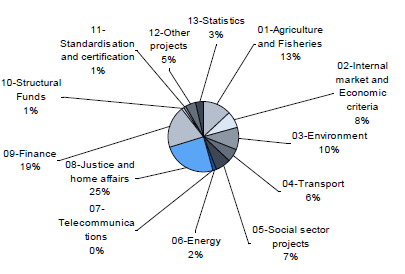
\includegraphics[width=4.5in]{Material/TwinningProjects}\\
Quelle: \cite{epec11}: 8.
\end{figure}
Die Grafik zeigt, dass der Anteil von Justice und Home Affairs 25\% an allen Twinning- und Twinning-Light-Projekten ausmachte. Überträgt man dies auf die in den Untersuchungsländern durchgeführten Projekte für die Jahre 2005-2008 (siehe Tabelle \ref{tab:AnteilTwinning}), kommt man auf maximal 3 Projekte pro Untersuchungsland, die dem Bereich Justice and Home Affairs zugeordnet sind. Es kann davon ausgegangen werden, dass es sich nicht in allen Fällen um Projekte zur Verwaltungsmodernisierung handelte, da auch die Modernisierung des Justizsystems unter diese Kategorie fällt. Für die Untersuchungsländer kann also festgehalten werden, dass Twinning, eines der Instrumente, das für Verwaltungsmodernisierung als besonders angemessen eingeschätzt wird, zumindest für die Zeit von 2005-2008 nur in geringem Umfang zum Einsatz kam.
\subsection{IPA – Instrument für Pre-Accession Assistance}
Das Programm IPA ersetzt die bis 2006 geltenden Instrumente PHARE, ISPA,\footnote{ISPA: Instrument for Structural Policies for Pre-Accession.} SAPARD,\footnote{SAPARD: Special Accession Programme for Agriculture \& Rural Development.} Heranführungshilfe für die Türkei und CARDS. Damit ist IPA seitdem das zentrale Instrument der Heranführungshilfe für die Beitrittsländer und die potenziellen Beitrittsländer in dem Prozess der Angleichung an die Standards der Europäischen Union zur Erlangung der Beitrittsreife.\par

Insbesondere soll das Instrument dazu beitragen:
\begin{itemize} \itemsep1pt \parskip0pt \parsep0pt
\item „die Demokratie und Rechtsstaatlichkeit zu stärken,
\item die öffentliche Verwaltung zu reformieren,
\item Wirtschaftsreformen durchzuführen,
\item die Menschen- und Minderheitenrechte zu achten,
\item die Gleichstellung der Geschlechter zu achten,
\item die Entwicklung der Zivilgesellschaft voranzubringen,
\item die regionale Zusammenarbeit sowie Versöhnung und Wiederaufbau zu fördern“ (\cite{senatskanzlei}). 
\end{itemize}
Grundlage für die Entwicklung von Projekten im Rahmen des IPA-Programmes sind folgende Dokumente:
\begin{itemize} \itemsep1pt \parskip0pt \parsep0pt
\item die Erweiterungsstrategie der Europäischen Kommission;
\item die jährlichen Fortschrittsberichte von der Europäischen Kommission. Für jedes (potenzielle) Beitrittsland von der Europäischen Kommission erstellt;
\item die Accession Partnerships (vgl. \cite{eurcom11a}).
\end{itemize}
Auf Basis dieser Dokumente werden mittelfristige Planungsdokumente, sog. Mehrjahresprogramme (über 3–4 Jahre), für jedes Land bzw. für mehrere Länder erstellt, die eine grobe Mittelaufteilung ausweisen, und nach den jeweiligen Bedürfnissen jedes einzelnen Empfängerlandes für die fünf Komponenten des IPA-Instruments angepasst wurden:
\begin{enumerate}[label=IPA {\Roman*}:,align=left,  leftmargin=*] \itemsep1pt \parskip0pt \parsep0pt
\item Übergangshilfe und Institutionenaufbau
\item  grenzübergreifende Zusammenarbeit
\item regionale Entwicklung (nur für Beitrittsländer)
\item Entwicklung der Humanressourcen (nur für Beitrittsländer)
\item ländliche Entwicklung (nur für Beitrittsländer)
\end{enumerate}
Die Komponenten I und II werden durch die Kommission selbst oder durch die Delegationen der Kommission in den Empfängerländern verwaltet. Die Komponenten III bis V stehen nur den Beitrittsländern zur Verfügung und werden nach den Prinzipien der Strukturfondsförderung in den Empfängerländern mit den entsprechenden Verwaltungsstrukturen abgewickelt. Verwaltungsaufbau und -modernisierung fallen unter Institutionenaufbau, also IPA I, und können durch das IPA-Programm in den drei Untersuchungsländern gefördert werden.\par
Neben der Förderung von Projekten in den einzelnen Ländern können auch länderübergreifende Programme im Rahmen von IPA umgesetzt werden. Aus der folgenden Tabelle wird die Finanzplanung pro Sektor für diese länderübergreifenden Programme deutlich:
\begin{table}[H]

\caption{Mehrjähriger indikativer Finanzrahmenplan 2011–2013, länderübergreifend.}
\small
\begin{tabular}{|L{56mm}|R{25mm}|R{25mm}|R{25mm}|}\hline
\multicolumn{4}{ |l| }{{\bf Indikative finanzielle Zuwendung pro Sektor (in Millionen EUR)}}\\\hline
&{\bf2007–2010}&\multicolumn{2}{c|}{\bf 2010–2013}\\\hline
Justiz und Innere Angelegenheiten, inkl. Grundrechte und vulnerable groups &285&24&4,61\%\\\hline
Öffentliche Verwaltung&60,92&38,5&7,39\%\\\hline
Zivilgesellschaft&40,5&30&5,76\%\\\hline
Entwicklung des privaten Sektors&123,9&70&13,44\%\\\hline
Transport und Energie Infrastruktur, inkl. Nukleare Sicherheit&124,45&108&20,73\%\\\hline
Umwelt und Klimawandel&16,3&17&3,26\%\\\hline
Soziale Entwicklung &71,98&96,5&18,52\%\\\hline
Andere Investitionen&173,86&96&18,43\%\\\hline
Reserve&0&40,97&7,86\%\\\hline
{\bf Gesamt}&{\bf 640,41}&{\bf 502,97}&{\bf 100\%}\\\hline
\multicolumn{4}{c}{}\\
\multicolumn{4}{c}{\normalsize Quelle: \cite{eurcom11b}: 15 (eigene Übersetzung aus dem Englischen).}
\end{tabular}
\\
\end{table}

Aus dieser Tabelle wird ersichtlich, dass für regionale, also länderübergreifende Programme im Bereich der öffentlichen Verwaltung für den Zeitraum 2011–13 Mittel in Höhe von 24 Millionen Euro zur Verfügung stehen. Diese werden im Balkan vor allem für die Unterstützung der regionalen Trainingseinrichtung für die öffentliche Verwaltung verwendet, die Regional School for Public Administration (RESPA), die 2010 in Montenegro eröffnet wurde.\par

„Gemäß den in den Mehrjahresprogrammen festgelegten Prioritäten werden für jedes Land in jährlichen Programmen konkret die Ziele, die Interventionsbereiche, die erwarteten Ergebnisse, die Verwaltungsverfahren und der für die Finanzierung vorgesehene Gesamtbetrag, eine Kurzbeschreibung der Art der zu finanzierenden Vorhaben, Angaben über die vorgesehenen Beträge je Vorhaben und ein vorläufiger Durchführungszeitplan festgelegt. Sobald die Programme im nicht-öffentlichen IPA-Programmausschuss durch die Vertreter der EU-Mitgliedstaaten genehmigt sind, erfolgen die Ausschreibungen.“\footnote{http://ec.europa.eu/enlargement/pdf/countries/ipa\_miff\_081106\_en.pdf (Aufgerufen 11.12.2012).}

Die Förderung durch IPA kann unterschiedliche Formen annehmen; dies sind vor allem:
\begin{itemize} \itemsep1pt \parskip0pt \parsep0pt
\item Zuschüsse zu öffentlichen Investitionen;
\item Unterstützung von Projekten der Zivilgesellschaft;
\item Twinning;
\item Direkte Budgethilfe (in Ausnahmefällen und unter Überwachung);
\item Technische Hilfe (\cite{epec11}: 2).
\end{itemize}
Für den Zeitraum 2007–2013 sind insgesamt Mittel in Höhe von 11,565 Milliarden Euro vorgesehen (\cite{senatskanzlei}).\par


Für den Bereich Institutionenbildung, unter den die Verwaltungsmodernisierung fällt, sind folgende Ausgaben in den Untersuchungsländern vorgesehen. 
\begin{table}[H]
\centering

\caption{ IPA 2007-13 Übergangshilfe und Institutionenaufbau (in Euro)}
\small
\begin{tabular}{|L{12mm}|R{16mm}|R{16mm}|R{16mm}|R{16mm}|R{16mm}|R{16mm}|R{16mm}|}\hline
&2007&
2008&
2009&
2010&
2011&
2012&
2013\\\hline
Maze\-donien&
41.641.613&
41.122.001&
39.328.499&
36.317.068&
28.803.410&
28.207.479&
27.941.228\\\hline
Monte\-negro&
27.490.504&
28.112.552&
28.632.179&
29.238.823&
29.843.599&
30.446.471&
30.996.035\\\hline
Alba\-nien&
54.318.790&
62.117.756&
71.377.079&
82.711.421&
84.301.650&
85.987.683&
87.446.037\\\hline
\multicolumn{8}{c}{}\\
\multicolumn{8}{c}{\normalsize Quelle: \cite{eurcom09b}.}
\end{tabular}
\end{table}
In einer Studie zur Implementierung von IPA-Funds kommen die Autoren eines Think Tank in Mazedonien zu dem Ergebnis: „So far, it has been a general rule that the key roles in IPA program management for WB countries are fulfilled jointly by the central governments and the EU delegations to these countries. It has been observed that the participation of local authorities and Civil Society Organisations (CSOs) in the process of designing IPA priorities and drafting the national or local strategic documents has been limited. All WB candidate countries have encountered some common difficulties in dealing with IPA rules” (\cite{eurmov10}: 4).\par
Eine Studie zur Effektivität des IPA-Instrumentes, im Auftrag der EU durchgeführt, konstatiert die Erfolge des Instruments vor allem für Bereiche, die konkret im Acquis geregelt sind: „Effectiveness was judged to be strongest in those areas where actions are related to the alignment/adoption of the acquis, notably where the acquis is clearly defined in terms of a legal and administrative framework to be achieved”. Themen, die nicht konkret im Acquis definiert sind, so auch die Reform der öffentlichen Verwaltung, sehen die Evaluatoren das IPA-Programm kritischer: „Where the acquis is defined in a looser framework or there is not a formal acquis chapter (e.g. public administration), effectiveness is less evident. For this type of interventions the BENF needs to establish its own, appropriate strategic/implementation frameworks, often involving interagency cooperation” (\cite{htspe}: 37).\par
Eine andere Analyse des bisherigen IPA-Programmes gibt zu bedenken, dass schwache administrative Kapazitäten in den Kandidaten- und potenziellen Kandidatenländern dazu führen können, Ressourcen zu binden, die anderswo nötiger und effektiver eingesetzt werden könnten: „Given the weak economic conditions, relatively fragile governance and underdeveloped administrative capacities in some beneficiaries, adopting EU standards at this stage may add significant costs to public activities and can inhibit the short-term competitiveness of productive activities” (\cite{epec11}: 3).\par
Eine weitere Problematik im Zusammenhang mit der IPA-Förderung generell, aber besonders für kleinere Länder, wird in einer Entschließung des Europäischen Parlaments von 2011 zu Montenegro deutlich: „Das Europäische Parlament nimmt mit Zufriedenheit zur Kenntnis, dass die IPA-Hilfe in Montenegro gut funktioniert; fordert sowohl die Regierung Montenegros als auch die Kommission auf, das Verwaltungsverfahren für die Beantragung von IPA-Mitteln zu vereinfachen, damit diese für kleinere und dezentral organisierte Bürgerorganisationen, Gewerkschaften und andere Empfänger einfacher zugänglich sind“ (\cite{eurpar11}: o.S.). 

\subsection{Die SIGMA-Initiative der OECD }
\label{subsec:Die SIGMA-Initiative der OECD}

Von besonderer Bedeutung im Hinblick auf das Thema „Administrative Kapazitäten von Kandidatenländern“ ist die gemeinsame Initiative der Organisation für Ökonomische Zusammenarbeit und Entwicklung (OECD) und der Europäischen Kommission mit dem SIGMA-Programm (Support for Improvement in Governance and Management). SIGMA wurde 1992 gegründet, co-finanziert durch die EU. Ziel war es, die Länder Mittel- und Osteuropas bei der Modernisierung ihrer öffentlichen Verwaltungen zu unterstützen. In den späten 1990er Jahren entwickelte SIGMA Baseline-Kriterien, die Grundlage sind für die Betrachtung und Beurteilung der horizontalen administrativen Kapazitäten der Kandidatenländer. Diese OECD/SIGMA Baseline-Kriterien für die öffentliche Verwaltung sind: 
\begin{enumerate} \itemsep1pt \parskip0pt \parsep0pt
\item Policy-Entwicklung und Koordination 
\item Civil service und Verwaltungsrecht
\item Management der öffentlichen Ausgaben
\item Beschaffungswesen im öffentlichen Bereich
\item Interne Finanzkontrolle
\item Externe Rechnungsprüfung (vgl. \cite{cardona09}: 3).
\end{enumerate}
In der Arbeit legt SIGMA besonderen Wert darauf, den Austausch und die Zusammenarbeit von Regierungen zur Verwaltungsentwicklung zu fördern. Dazu gehört u.a. logistische Unterstützung für die Gründung von Netzwerken regionaler Verwaltungsspezialisten in Mittel- und Osteuropa und der Austausch dieser Experten mit solchen aus etablierten Demokratien. Weiterhin werden Informationsmaterial und Berichte über bestimmte Themen und Länder auf der OECD/SIGMA-Website veröffentlicht. Es geht darum:
\begin{itemize} \itemsep1pt \parskip0pt \parsep0pt
\item den Reformfortschritt zu messen und Prioritäten zu identifizieren anhand guter Europäischer Praxis und bestehendem EU-Recht (Acquis communautaire). 
\item Unterstützung für Entscheidungsträger und Administratoren zur Verfügung zu stellen, für die Einrichtung der rechtlichen Rahmenbedingungen und Prozesse, um europäischen Standards und guter Praxis zu entsprechen.
\item EU-Finanzierung durch Hilfe beim Projektdesign und der Implementierung zu unterstützen (vgl. \cite{oecd99}: 2).
\end{itemize}
SIGMA veröffentlicht seit 1999 Länderberichte zu bestimmten Themen der Verwaltungsentwicklung. Diese werden von der Europäischen Kommission für ihre jährlichen Fortschrittsberichte zu den Kandidaten- und potenziellen Kandidatenländern verwendet.\par
Ohne konkretes EU-Modell zur Verwaltungsmodernisierung füllte die SIGMA-Initiative in gewisser Weise das Vakuum, das aufgrund fehlender klarer Bestimmungen auf EU-Ebene und der sich entwickelnden Konditionalität im administrativen Bereich entstanden war. Da die EU im Rahmen der Konditionalität kein allgemein gültiges Modell der öffentlichen Verwaltung zugrunde legt, bleibt es bei der allgemeinen Forderung der „ability to implement the acquis“. Dimitrova kritisiert, dass die EU nicht das Modell des New Public Management (NPM) zugrunde legt, das einflussreichste Paradigma der letzten Jahrzehnte in der Debatte um Verwaltungsmodernisierung. Stattdessen dient der EU ein weitgehend klassisches Weberianisches Modell der Bürokratie mit Etablierung eines professionellen (Berufs-) Beamtenapparates, der politisch unabhängig ist, als wesentlicher Orientierungspunkt (vgl. \cite{dimit05}: 81).

\subsection{Abgeschlossene Programme für den Westbalkan}
Herausragende bereits abgeschlossene Programme zur Heranführung beitrittswilliger Staaten an die EU-Standards sind die Tätigkeit der European Agency for Reconstruction (EAR) sowie die Programme PHARE und CARDS, die nachfolgend jeweils bezüglich der Verwaltungsmodernisierung kurz dargestellt werden.

\subsubsection{European Agency for Reconstruction}
Die European Agency for Reconstruction war für die Verwaltung der wesentlichen Unterstützungsprogramme der EU für Serbien, Kosovo (unter UN-Verwaltung), Montenegro und Mazedonien zuständig. Die EAR wurde gegründet, um die Wiederaufbauhilfe der EU für Kosovo zu koordinieren. Nach dem Fall des Milosevic-Regimes im Jahr 2000 wurde das Mandat auf Serbien und Montenegro und 2002 auf Mazedonien erweitert. Die EAR hatte ihre Zentrale in Thessaloniki (Griechenland) und Büros in Pristina (Kosovo), Belgrad (Serbien), Podgorica (Montenegro) und Skopje (Mazedonien). Bis zum Juli 2007 hat die EAR ca. 2,3 Milliarden Euro an Hilfe in den von ihr unterstützten Ländern ausgezahlt, wie aus folgender Tabelle hervorgeht:
\renewcommand{\arraystretch}{1}
\begin{table}[H]
\center
\setlength\belowcaptionskip{10pt}
\caption{Die Agency for Reconstruction (EAR). Zuwendungen bis Ende Juli 2007}
\small
\begin{tabular}{|L{25mm}|R{36mm}|R{36mm}|R{16mm}|}\hline
&
Bereitgestellt&
Ausgezahlt&
Quote\\\hline
Serbien&
1,3 Milliarden Euro&
921 Millionen Euro&
71\%\\\hline
Montenegro&
130 Millionen Euro&
104 Millionen Euro&
80\%\\\hline
Kosovo&
1,11 Milliarden Euro&
998 Millionen Euro&
90\%\\\hline
Mazedonien&
327 Millionen Euro&
259 Millionen Euro&
79\%\\\hline
Gesamt EAR&
2,86 Milliarden Euro&
2,3 Milliarden Euro&
80\%\\\hline
\multicolumn{4}{c}{}\\
\multicolumn{4}{c}{{\normalsize Quelle: \cite{zink}: 8 (eigene Übersetzung aus dem Englischen).}}
\end{tabular}
\end{table}
Aus dieser Tabelle ist ersichtlich, dass der überwiegende Teil der durch die EAR ausgezahlten Hilfe dem Kosovo zugute kam. Neben den Hauptempfängerländern Kosovo und Serbien erhielten Mazedonien und Montenegro 259 und 104 Millionen Euro respektive an Hilfsleistungen.\par
Außer zum Wiederaufbau hat die EAR im Laufe der Zeit auch für andere Bereiche Unterstützung zur Verfügung gestellt, z.B. für Projekte zur wirtschaftlichen Entwicklung, zur Stabilisierung der administrativen Kapazitäten der geförderten Länder, im Justizsektor, der Zivilgesellschaft und im Bereich der Medien. Die EAR war dem Europäischen Parlament und dem Rat der Europäischen Union verantwortlich und arbeitete eng mit der Europäischen Kommission und ihren Vertretungen vor Ort zusammen. Im Dezember 2008 endete das Mandat der EAR und die Weiterführung der Förderprogramme ging an die EU-Delegationen in den unterstützen Ländern über (vgl. \cite{zink}: 10).

\subsubsection{PHARE}
Als Hauptinstrument der EU zur Heranführung der Kandidatenländer aus Zentral- und Osteuropa an die EU diente das PHARE-Programm.\footnote{Le phare (franz.) bedeutet Leuchtturm.} Dieses Programm war ursprünglich entwickelt worden, um Polen und Ungarn in Form von Wirtschaftshilfe bei der ökonomischen Umstrukturierung zu helfen, wurde aber später auf die anderen Beitrittskandidaten ausgedehnt (Bulgarien, Tschechische Republik, Estland, Lettland, Litauen, Slowakei, Slowenien und Rumänien). Einige Pilotprojekte in Polen und Ungarn zwischen 1995 und 1997 betrafen auch schon die administrative Kompetenz (\cite{tomtul}: 380). In einer schrittweise sich entwickelnden Heranführungsstrategie standen ab 1996 PHARE, Beitrittspartnerschaften, und nationale Programme für die Anpassung an den Acquis zur Verfügung. Seit dieser Zeit waren neben der Infrastruktur, rechtlicher und ökonomischer Angleichung auch die administrativen Kapazitäten der Beitrittsländer im Blick der EU. 1997 beschloss die EU-Kommission die „Agenda 2000“ und schlug vor, die Hilfen zu 30\% für Institutionenbildung und 70\% für Investitionen zur Verfügung zu stellen. Die Abordnung nationaler Experten der Kandidatenländer zu Schulungszwecken (TAIEX) und von Beamten der EU-Mitgliedsländer in die Kandidatenstaaten (Twinning) wurde als Instrument der Verwaltungsentwicklung und -unterstützung entwickelt (\cite{lipumb04}: 60).\par

Als Ziele des PHARE-Programmes nennt die EU auf ihrer Website:
\begin{itemize}
\item „helping the administrations of the candidate countries to acquire the capacity to implement the Community acquis. PHARE also helps the national and regional administrations, as well as regulatory and supervisory bodies, in the candidate countries to familiarise themselves with Community objectives and procedures;
\item helping the candidate countries to bring their industries and basic infrastructure up to Community standards by mobilising the investment required, particularly in areas where Community rules are increasingly demanding: environment, transport, industry, product quality, working conditions etc.”\footnote{http://europa.eu/legislation\_summaries/enlargement/2004\_and\_2007\_enlargement/e50004\_en.htm (Aufgerufen: 19.8.2012).}
\end{itemize}
In einer Evaluierung von PHARE-Projekten zur Verwaltungsmodernisierung in fünf Beitrittsländern\footnote{Estland, Lettland, Litauen, Polen und Slowakei.} wurden Projekte aus den Bereichen gesetzgeberische und organisatorische Reformen des civil service, Training für öffentlich Bedienstete und Verbesserung der IT-Infrastruktur untersucht. Die Ergebnisse sind schematisch in folgender Tabelle dargestellt:
\renewcommand{\arraystretch}{1}
 \begin{table}[H]
\center

\caption{Evaluierung von PHARE-Projekten zur Verwaltungsmodernisierung in CEE}
\small
\begin{tabular}{|L{40mm}|C{14mm}|C{14mm}|C{14mm}|C{14mm}|C{14mm}|C{14mm}|}\hline
&Anzahl Projekte&Efficiency&Effectiveness&Impact&Nachhaltigkeit&Durchschnitt\\\hline\hline
{\bf Land}&\multicolumn{6}{|r|}{}\\\hline
Estland&3&2,3&2,3&2&1,7&2,1\\\hline
Lettland&9&3,6&3,2&2,9&2,3&3\\\hline
Litauen&10&2,7&2,1&1,8&1,5&2\\\hline
Polen&15&3,8&3,5&2,3&2,1&3\\\hline
Slowakei&3&3&2,7&2,7&2,3&2,7\\\hline\hline
{\bf Projektarten}&\multicolumn{6}{|r|}{}\\\hline
Rechtliche und orga- nisatorische Reformen&30&3,3&2,9&2,3&1,9&2,6\\\hline
Weiterbildung/Training&5&3,6&3,4&3,2&3&3,3\\\hline
Informationstechnologie&5&3,2&2,8&1,8&1,6&2,4\\\hline\hline
{\bf Zuwendungs-\newline empfänger}&\multicolumn{6}{|r|}{}\\\hline
Zentrale Exekutive&18&2,9&2,1&1,8&1,7&2,1\\\hline
Lokale Exekutive&13&3,7&3,7&2,8&2,2&3,1\\\hline
Lokale und Zentrale Exekutive&6&3,5&3,5&2,5&2,2&2,9\\\hline
Parlament&3&3,7&3,7&2,7&2,7&3,2\\\hline\hline
{\bf Durchschnitt (alle Projekte)}&40&3,3&3&2,3&2&2,6\\\hline\hline
\multicolumn{7}{|r|}{1 (sehr schlecht), 2 (eher schlecht), 3 (angemessen), 4 (gut), 5 (sehr gut)}\\\hline
\multicolumn{7}{c}{}\\
\multicolumn{7}{c}{\normalsize Quelle: \cite{ips}: 96}\\
\multicolumn{7}{c}{ (\normalsize eigene Übersetzung aus dem Englischen).}
\end{tabular}
\end{table}
\renewcommand{\arraystretch}{1.2}

Aus dieser Tabelle ist ersichtlich, dass im Bereich der größten Anzahl der Projekte, bei rechtlichen und organisatorischen Reformen des civil service (30 Projekte), die Nachhaltigkeit nicht ausreichend gegeben war.

Zur Analyse der Gründe für das generell schlechte Abschneiden der untersuchten Projekte werden mehrere Faktoren benannt. Ein wesentlicher Faktor wird von den Evaluatoren darin gesehen, dass es entweder keine strategische Ausrichtung der PAR-Projekte gab, oder diese häufigen Veränderungen unterlag. Weiterhin war die Projektentwicklung oft extern vergeben und hat die konkreten Bedingungen vor Ort nicht ausreichend berücksichtigt. Die Auswahl der Projekte war ad-hoc und „demand driven“, PAR war dagegen „project driven” mit starkem Gewicht auf inputs (Unterstützung durch Experten und Bereitstellung von Equipment) und wenig Augenmerk auf outputs und impact. Während die Autoren der Evaluierung viele der identifizierten Probleme den Turbulenzen der frühen Jahre der Transition zurechnen, mahnen sie Verbesserungen im Management der Unterstützungsprogramme an (vgl. \cite{ips}: 98).

Die Autoren der Evaluation schließen mit einer Empfehlung an die EU-Kommission: 

„The Commission is urgently in need of some criteria:
\begin{itemize}
\item against which a rational discussion of PAR issues can be held, even if these discussions cannot form a formal part of the accession negotiations;
\item that would offer some guidance and policy focus for PHARE PAR programmes” (\cite{ips}: 103).
\end{itemize}
Für die Länder des Westbalkans wurde das PHARE-Programm im Jahr 2000 durch ein neues Instrument, CARDS, abgelöst.


\subsubsection{CARDS} 

Die wirtschaftliche, politische und soziale Zusammenarbeit der EU mit den Ländern des Westlichen Balkans wurde mit dem Hilfsprogramm „Community Assistance for Reconstruction, Democratization and Stabilization“ (CARDS) als neuem Instrument umgesetzt. CARDS war Teil der Stabilisierungs- und Assoziierungsstrategie der Europäischen Union gegenüber dem Westlichen Balkan, und im Rahmen des SAP wurden Mittel unter CARDS abrufbar. Ab dem Jahr 2000 wurden Mittel der EU bereitgestellt, um Reformprozesse in den Zielländern zu unterstützen (vgl. \cite{calic01}: 12).\par

Die drei Untersuchungsländer der vorliegenden Arbeit (Albanien, Mazedonien und Montenegro) profitierten ab 2000 von CARDS, das bis 2006 zur Verfügung stand. Die Zuständigkeit für das CARDS-Programm wechselte im Jahr 2005 von einer gemeinsamen Zuständigkeit der Generaldirektion Außenbeziehungen und des Europäischen Amtes für Entwicklungszusammenarbeit „EuropeAid“ hin zur Generaldirektion Erweiterung (vgl. \cite{eurrh}: C285/5).\par
Die Gelder aus dem CARDS-Programm standen für verschiedenste Zwecke zur Verfügung, z.B. für Infrastrukturprojekte, Hilfe für Flüchtlinge, Institutionenbildung und Polizeikooperation. Fast die Hälfte des Geldes war für Serbien/Montenegro bestimmt, vor allem aufgrund der Situation im Kosovo. In Mazedonien und Montenegro war ab 2003 die European Agency for Reconstruction (EAR) für die Verwaltung des Programmes zuständig. In Albanien wurde CARDS von der Delegation der Europäischen Kommission in Tirana verwaltet. Regionale Projekte wurden direkt von Brüssel unterstützt. Der Anteil des tatsächlich verausgabten Geldes unterscheidet sich für die Untersuchungsländer. Montenegro hatte eine Absorptionsrate von 86\%, Mazedonien 52\% und Albanien rangiert am unteren Ende mit 29\%. (vgl. \cite{inotai}: 42). Insgesamt wurden von der EU in den Jahren 2000–2006 unter CARDS 4,6 Milliarden Euro zur Verfügung gestellt (vgl. \cite{mus}: 13). Der Europäische Rechnungshof kommt in einer Evaluierung des CARDS-Programmes zu dem Ergebnis, dass vor allem Infrastrukturmaßnahmen erfolgreich umgesetzt wurden, während CARDS bei der Verbesserung der staatlichen Verwaltungskapazitäten weniger effektiv war. Gründe werden vor allem darin gesehen, dass der Schwerpunkt ursprünglich nicht auf dem Institutionenaufbau lag und die Empfängerländer keine ausreichenden Kapazitäten zur Absorption der Hilfe hatten (vgl. \cite{eurrh}: C285/15).
\begin{table}[H]

\center
\caption{CARDS Mittelzuweisungen Albanien, Mazedonien (2002-2006) und Montenegro (2005-2006), nach Sektoren in Millionen Euro}
\small
\begin{tabular}{|L{60mm}|R{13mm}|R{13mm}|R{13mm}|R{13mm}|}\hline
{\bf Albanien} &{\bf 2002} &{\bf 2003} &{\bf 2004} &{\bf 2005-6}\\\hline
Justice \& Home Affairs&21&20&35&27\\
Administrative Capacity Building&6&8&4&23\\
Economic \& Social Development&12,9&17,5&12&31\\
Environment, Natural Resources&4&-&10&-\\
Democratic Stabilisation&1&1&2,5&4\\\hline
\end{tabular}
\begin{tabular}{|L{60mm}|R{13mm}|R{13mm}|R{13mm}|R{13mm}|}\hline
{\bf Mazedonien} &{\bf 2002} &{\bf 2003} &{\bf 2004} &{\bf 2005-6}\\\hline
Justice \& Home Affairs&7&12,5&24&17\\
Administrative Capacity Building&14&9&8,5&24\\
Economic \& Social Development&11,5&11&15&20\\
Environment, Natural Resources&-&1&2&3\\
Democratic Stabilisation&3&3&3&2\\\hline
\end{tabular}
\begin{tabular}{|L{60mm}|R{13mm}|R{13mm}R{13mm}R{13mm}}\cline{1-2}
{\bf Montenegro} &{\bf 2005-6}\\\cline{1-2}
Justice \& Home Affairs&3&&&\\
Administrative Capacity Building&11&&&\\
Economic \& Social Development&16,3&&&\\
Environment, Natural Resources&6&&&\\
Democratic Stabilisation&3,7&&&\\\cline{1-2}
\multicolumn{5}{c}{}\\
\multicolumn{5}{C{114mm}}{Quelle: http://ec.europa.eu/enlargement/how-does-it-work/}\\
\multicolumn{5}{C{114mm}}{financial-assistance/cards/statistics2000-2006\_en.htm}\\
\multicolumn{5}{C{114mm}}{ (Aufgerufen: 5.5.2010).}
\end{tabular}
\end{table}

Aus den Tabellen wird deutlich, dass in den beiden Jahren 2005 und 2006 in Albanien und Mazedonien ein starker Anstieg der Ausgaben im Bereich Administrative Capacity Building stattgefunden hat. In einer Evaluation des CARDS-Programmes für Albanien wird dennoch konstatiert, dass die Erfolge des Programmes im Bereich Verwaltungsunterstützung moderat waren: „Support to public administration has been limited in terms of both the number of projects and project size, and a proprer public administration reform and civil service reform have not been implemented“ (\cite{cowi}: ii). Für Montenegro ist die Darstellungsweise erst ab 2005/6 gegeben, wohl aufgrund der Darstellung zusammen mit Serbien bis zur staatlichen Unabhängigkeit 2006. 

\subsection{Zwischenergebnis für die Verwaltungsmodernisierung}
Betrachtet man die theoretischen Ansätze, die praktische Entwicklung und die gezielten Förderprogramme im Zusammenhang, so wird erkennbar, dass trotz der Erfahrungen der EU mit der Osterweiterung die Verwaltungsmodernisierung und der Status der Verwaltung in den Beitrittsländern nicht angemessen berücksichtigt wird. In den Förderprogrammen für den Westlichen Balkan werden regelmäßig Mittel auch für die Modernisierung der öffentlichen Verwaltung bereitgestellt. In Abwesenheit einer glaubhaften Konditionalität und einer Verankerung des Themas im Acquis communautaire sind kritische Evaluationen der bisherigen Förderprogramme in Bezug auf Verwaltungsentwicklung im Balkan allerdings nicht verwunderlich. Es entsteht der Eindruck, dass die EU die Verwaltungsmodernisierung zwar immer wieder als wichtig bezeichnet, z.B. in den jährlichen Fortschrittsberichten, aber keine operationalisierbaren Instrumente zu einer nachhaltigen Förderung einer modernen Verwaltung entwickelt hat. \par
Dies ist umso erstaunlicher, als die fehlende Modernisierung der öffentlichen Verwaltung in den Ländern der letzten Erweiterungswelle, wie gezeigt wurde, von der Forschung deutlich herausgearbeitet wurde.\par
Um ein möglichst genaues Bild des Status quo der Verwaltungsentwicklung in den drei Untersuchungsländern zu erhalten, wird im Folgenden der Blick erweitert um die historische Entwicklung der öffentlichen Verwaltung.



